%=======================================================================
%  TARVI — Methodology Notes
%  A self-contained technical companion: from the splicing ODE to
%  velocity, latent time, and the training objective.
%
%  Compile with:  pdflatex TARVI_methodology_notes.tex   (twice, for refs)
%  Packages used are all part of a standard TeX Live / MiKTeX install.
%=======================================================================
\documentclass[11pt,a4paper]{article}

\usepackage[T1]{fontenc}
\usepackage[utf8]{inputenc}
\usepackage[margin=2.6cm]{geometry}
\usepackage{amsmath,amssymb,amsthm}
\usepackage{booktabs}
\usepackage{array}
\usepackage{graphicx}
\usepackage{xcolor}
\usepackage{framed}
\usepackage{enumitem}
\usepackage{listings}
\usepackage{caption}
\usepackage{tikz}
\usepackage{pgfplots}
\pgfplotsset{compat=1.18}
\usetikzlibrary{arrows.meta,positioning,calc,fit,backgrounds,decorations.pathreplacing}
\usepackage[hidelinks]{hyperref}

%----------------------------- styling --------------------------------
\definecolor{tarvinavy}{RGB}{26,58,92}
\definecolor{shadecolor}{RGB}{244,247,250}
\definecolor{codegray}{RGB}{100,100,100}
\definecolor{codekw}{RGB}{0,90,160}
\definecolor{cU}{RGB}{198,90,20}      % unspliced
\definecolor{cS}{RGB}{31,95,155}      % spliced
\definecolor{cGrey}{RGB}{130,130,130}
\definecolor{cGreen}{RGB}{40,125,80}
\definecolor{cRed}{RGB}{175,45,45}

%----------------------------- figure styles --------------------------
\pgfplotsset{
  tarviaxis/.style={
    width=0.52\textwidth, height=0.38\textwidth,
    axis lines=left,
    tick align=outside,
    tick label style={font=\scriptsize},
    label style={font=\small},
    legend style={font=\scriptsize, draw=none, fill=none},
    every axis plot/.append style={line width=1pt},
    grid=major, grid style={line width=0.3pt, draw=lightgray!50},
  }
}

\tikzset{
  blk/.style={draw=tarvinavy, fill=tarvinavy!6, rounded corners=2pt,
              align=center, font=\footnotesize, inner sep=4pt, minimum height=7mm},
  dat/.style={draw=cGrey, fill=gray!8, rounded corners=2pt,
              align=center, font=\footnotesize, inner sep=4pt, minimum height=7mm},
  fix/.style={draw=cGreen, fill=cGreen!8, rounded corners=2pt,
              align=center, font=\footnotesize, inner sep=4pt, minimum height=7mm},
  ar/.style={-{Stealth[length=2mm]}, draw=tarvinavy, line width=0.7pt},
  arg/.style={-{Stealth[length=2mm]}, draw=cRed, line width=0.7pt, dashed},
}

\newenvironment{keybox}{\begin{shaded}\noindent}{\end{shaded}}

\lstset{
  basicstyle=\ttfamily\small,
  keywordstyle=\color{codekw}\bfseries,
  commentstyle=\color{codegray}\itshape,
  stringstyle=\color{tarvinavy},
  showstringspaces=false,
  breaklines=true,
  frame=single,
  rulecolor=\color{lightgray},
  xleftmargin=0.5em,
  language=Python,
}

\newcommand{\uns}{u}
\newcommand{\spl}{s}
\newcommand{\ts}{t_{s}}
\newcommand{\tmax}{t_{\max}}
\newcommand{\R}{\mathbb{R}}
\newcommand{\E}{\mathbb{E}}
\newcommand{\sg}{\operatorname{sg}}
\newcommand{\softplus}{\operatorname{softplus}}

\theoremstyle{definition}
\newtheorem{prop}{Proposition}

\title{\textbf{TARVI: Methodology Notes}\\[0.3em]
\large From the splicing ODE to velocity, latent time, and the training objective}
\author{Technical companion document}
\date{}

%======================================================================
\begin{document}
\maketitle

\begin{abstract}
\noindent
These notes give a self-contained account of how TARVI works: the biophysical
model it rests on, the exact solutions of that model, what the data can and
cannot identify, how the neural architecture is organised, how the model is
trained without any ground-truth velocity, and how velocity and latent time
are finally computed. Every equation is derived rather than quoted, and every
component is tied back to the code that implements it. The document is
intended to answer, in one place, the questions that arise naturally when
reading the implementation --- in particular: \emph{where do the equations come
from}, \emph{how are unknown kinetic rates obtained}, \emph{why is there an
encoder and decoder at all}, and \emph{what is the loss computed against when
no ground truth exists}.
\end{abstract}

\tableofcontents
\newpage

%======================================================================
\section{Introduction}
%======================================================================

\subsection{What RNA velocity is}

Messenger RNA passes through a short pipeline inside every cell. A gene is
transcribed into unspliced pre-mRNA, introns are spliced out to give mature
mRNA, and mature mRNA is eventually degraded:
%
\begin{equation}
\text{gene} \;\xrightarrow{\;\alpha\;}\; \underbrace{u}_{\text{unspliced}}
\;\xrightarrow{\;\beta\;}\; \underbrace{s}_{\text{spliced}}
\;\xrightarrow{\;\gamma\;}\; \varnothing
\end{equation}
%
with three rate constants: $\alpha$ (transcription), $\beta$ (splicing) and
$\gamma$ (degradation of spliced mRNA). Note that \emph{translation does not
appear}. Protein is not measured in scRNA-seq, so it plays no role in the
model; $\gamma$ is a degradation rate, not a translation rate.

Modern droplet-based protocols report unspliced and spliced counts separately.
\emph{RNA velocity} is the instantaneous rate of change of the mature pool:
%
\begin{keybox}
\begin{equation}
v \;=\; \frac{d\spl}{dt} \;=\; \beta \uns - \gamma \spl
\label{eq:velocity}
\end{equation}
\emph{Mature mRNA rises when it arrives faster than it is destroyed.}
\end{keybox}
%
A positive $v$ means the gene is being switched on and the cell is moving
toward a state in which that gene is more highly expressed. Computing $v$ for
every gene yields one vector per cell --- an arrow pointing at the cell's near
future. Projected onto an embedding, those arrows reconstruct a
differentiation trajectory from a single static snapshot, with no time-course
experiment required.

\subsection{What TARVI adds}

Contemporary velocity estimators share three structural limitations, and
TARVI targets each one directly.

\begin{enumerate}[leftmargin=*]
\item \textbf{Static transcription rate.} The per-gene rate $\alpha_g$ is
      treated as a constant, ignoring that genes are switched on by
      transcription factors whose abundance differs from cell to cell. TARVI
      makes $\alpha$ \emph{cell-specific}, computed from a mask of known
      TF--target relationships derived from ENCODE ChIP-seq and ChEA.
\item \textbf{Weakly supervised latent time.} Latent time falls out of the fit
      with no direct signal, and is consequently poorly calibrated. TARVI adds
      a supervised residual time head trained by two complementary losses.
\item \textbf{Local/global mismatch.} Velocity is a local derivative;
      a trajectory is a global object. TARVI blends the learned time with
      diffusion pseudotime computed on the velocity transition graph.
\end{enumerate}

\subsection{How to read these notes}

Section~\ref{sec:kinetics} derives the kinetic model and its exact solutions
from first principles. Section~\ref{sec:identifiability} establishes what the
data can and cannot determine --- this underpins several later design choices
and is worth reading before the architecture. Section~\ref{sec:data} covers
data preparation. Section~\ref{sec:architecture} describes the network.
Section~\ref{sec:training} explains how training proceeds without ground truth.
Section~\ref{sec:inference} covers velocity and latent-time computation at
inference. Appendix~\ref{app:notation} is a notation and tensor-shape
reference; readers may find it useful to keep open alongside the text.

%======================================================================
\section{The kinetic model and its exact solutions}
\label{sec:kinetics}
%======================================================================

\subsection{Mass-action kinetics}

The three processes give a coupled pair of ordinary differential equations:
%
\begin{keybox}
\begin{align}
\frac{d\uns}{dt} &= \underbrace{\alpha}_{\text{transcribed}} \;-\; \underbrace{\beta \uns}_{\text{spliced away}}
\label{eq:ode-u}\\[0.4em]
\frac{d\spl}{dt} &= \underbrace{\beta \uns}_{\text{arrives}} \;-\; \underbrace{\gamma \spl}_{\text{degraded}}
\label{eq:ode-s}
\end{align}
\end{keybox}
%
The form of each term follows from elementary reaction kinetics:

\begin{itemize}[leftmargin=*]
\item $\alpha$ is a \emph{constant} (zeroth order): the rate at which
      polymerase produces transcripts does not depend on how much RNA is
      already present.
\item $\beta \uns$ is \emph{first order}: twice as much unspliced RNA means
      twice as many splicing events per unit time.
\item $\gamma \spl$ is likewise first order for degradation.
\end{itemize}

The coupling matters. The term $\beta \uns$ is subtracted in
\eqref{eq:ode-u} and added in \eqref{eq:ode-s}: nothing is lost in transit, it
is the same molecules moving from one pool to the other. This conservation is
what makes the unspliced pool a \emph{leading indicator} of the spliced pool,
and is the entire basis of RNA velocity.

\subsection{Induction: solving for \texorpdfstring{$u$}{u}}

Equation~\eqref{eq:ode-u} is a first-order linear ODE. Write it in standard
form and multiply by the integrating factor $e^{\beta t}$:
%
\begin{equation}
\frac{d\uns}{dt} + \beta \uns = \alpha
\qquad\Longrightarrow\qquad
e^{\beta t}\frac{d\uns}{dt} + \beta e^{\beta t}\uns = \alpha e^{\beta t}.
\end{equation}
%
The left-hand side is now exactly the product rule in reverse, so
%
\begin{equation}
\frac{d}{dt}\Big(\uns\, e^{\beta t}\Big) = \alpha e^{\beta t}.
\end{equation}
%
Integrating both sides and dividing through by $e^{\beta t}$,
%
\begin{equation}
\uns\, e^{\beta t} = \frac{\alpha}{\beta}e^{\beta t} + C
\qquad\Longrightarrow\qquad
\uns(t) = \frac{\alpha}{\beta} + C e^{-\beta t}.
\end{equation}
%
Imposing the induction initial condition $\uns(0) = 0$ (the gene starts from
off) gives $C = -\alpha/\beta$, hence
%
\begin{keybox}
\begin{equation}
\boxed{\;\uns(t) = \frac{\alpha}{\beta}\Big(1 - e^{-\beta t}\Big)\;}
\label{eq:u-ind}
\end{equation}
\end{keybox}
%
Two sanity checks: $\uns(0) = 0$ as required, and $\uns(t) \to \alpha/\beta$ as
$t \to \infty$, which is the steady-state level.

\subsection{Induction: solving for \texorpdfstring{$s$}{s}}

Substituting \eqref{eq:u-ind} into \eqref{eq:ode-s} gives a forced linear ODE
in $\spl$:
%
\begin{equation}
\frac{d\spl}{dt} + \gamma \spl
= \beta \cdot \frac{\alpha}{\beta}\Big(1 - e^{-\beta t}\Big)
= \alpha - \alpha e^{-\beta t}.
\end{equation}
%
Applying the integrating factor $e^{\gamma t}$,
%
\begin{equation}
\frac{d}{dt}\Big(\spl\, e^{\gamma t}\Big)
= \alpha e^{\gamma t} - \alpha e^{(\gamma - \beta) t},
\end{equation}
%
and integrating,
%
\begin{equation}
\spl\, e^{\gamma t}
= \frac{\alpha}{\gamma}e^{\gamma t}
- \frac{\alpha}{\gamma - \beta}e^{(\gamma - \beta)t} + C .
\end{equation}
%
Dividing by $e^{\gamma t}$ and imposing $\spl(0) = 0$, which fixes
$C = \frac{\alpha}{\gamma-\beta} - \frac{\alpha}{\gamma}$, and collecting terms:
%
\begin{keybox}
\begin{equation}
\boxed{\;\spl(t) = \frac{\alpha}{\gamma}\Big(1 - e^{-\gamma t}\Big)
+ \frac{\alpha}{\gamma - \beta}\Big(e^{-\gamma t} - e^{-\beta t}\Big)\;}
\label{eq:s-ind}
\end{equation}
\end{keybox}
%
Again $\spl(0) = 0 + \frac{\alpha}{\gamma-\beta}(1 - 1) = 0$, and
$\spl(t) \to \alpha/\gamma$ as $t \to \infty$.

The second term in \eqref{eq:s-ind} is the \textbf{lag term}. It is what makes
$\spl$ trail behind $\uns$, and therefore what makes the $(\spl,\uns)$ trajectory
trace a loop rather than a straight line. Everything downstream --- the
identifiability of the rates, the gene filter, the initialisation --- follows
from the existence of that lag.

\subsection{Repression}

At the switch time the gene is turned off, so $\alpha = 0$. The equations are
the same but with new initial conditions $(\uns_0, \spl_0)$, namely the values
reached at the end of induction. Equation \eqref{eq:ode-u} becomes pure decay:
%
\begin{equation}
\frac{d\uns}{dt} = -\beta \uns
\qquad\Longrightarrow\qquad
\boxed{\;\uns(t) = \uns_0\, e^{-\beta t}\;}
\label{eq:u-rep}
\end{equation}
%
For $\spl$, the forcing term is now $\beta \uns_0 e^{-\beta t}$:
%
\begin{equation}
\frac{d}{dt}\Big(\spl\, e^{\gamma t}\Big) = \beta \uns_0 e^{(\gamma - \beta)t}
\qquad\Longrightarrow\qquad
\spl(t) = \frac{\beta \uns_0}{\gamma - \beta}e^{-\beta t} + Ce^{-\gamma t}.
\end{equation}
%
Imposing $\spl(0) = \spl_0$ gives
$C = \spl_0 - \frac{\beta \uns_0}{\gamma - \beta}$, hence
%
\begin{keybox}
\begin{equation}
\boxed{\;\spl(t) = \spl_0 e^{-\gamma t}
- \frac{\beta \uns_0}{\gamma - \beta}\Big(e^{-\gamma t} - e^{-\beta t}\Big)\;}
\label{eq:s-rep}
\end{equation}
\end{keybox}

Equations \eqref{eq:u-ind}, \eqref{eq:s-ind}, \eqref{eq:u-rep} and
\eqref{eq:s-rep} are implemented term for term by the induction and repression
solvers in \texttt{tarvi/\_module.py}. Because they are closed-form, no
numerical integration is ever performed: evaluating the model at any time is a
handful of exponentials, fully differentiable and cheap.

\subsection{Steady states and the phase portrait}
\label{sec:steady}

Setting both derivatives to zero,
%
\begin{equation}
\alpha - \beta \uns^{*} = 0 \;\Rightarrow\; \uns^{*} = \frac{\alpha}{\beta},
\qquad
\beta \uns^{*} - \gamma \spl^{*} = 0 \;\Rightarrow\; \spl^{*} = \frac{\alpha}{\gamma}.
\end{equation}
%
These are the two \emph{steady} states of the four-state model: the induction
plateau $(\alpha/\beta,\ \alpha/\gamma)$ and, trivially, the repression floor
$(0, 0)$.

Dividing one by the other gives a relation that will recur throughout these
notes:
%
\begin{keybox}
\begin{equation}
\frac{\uns^{*}}{\spl^{*}} = \frac{\gamma}{\beta}
\label{eq:ss-slope}
\end{equation}
\emph{The steady-state slope of the phase portrait equals $\gamma/\beta$.}
\end{keybox}

The \textbf{phase portrait} is the scatter of $(\spl, \uns)$ across all cells for
a single gene. During induction $\uns$ rises first and $\spl$ lags, producing an
upper-left arm; during repression $\uns$ falls first and $\spl$ lags again,
producing a lower-right arm. Together they trace a counter-clockwise loop
whose diagonal has slope $\gamma/\beta$ by \eqref{eq:ss-slope}. This geometry
is the sole source of information about the kinetic rates, as
Section~\ref{sec:identifiability} makes precise.

Figure~\ref{fig:dynamics} shows both views of the same gene: the time courses on
the left, and the phase portrait they trace on the right.

\begin{figure}[htbp]
\centering
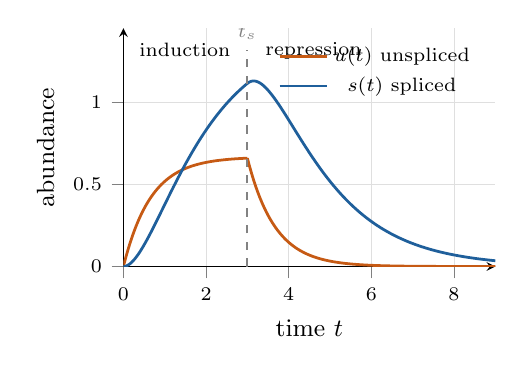
\begin{tikzpicture}
\begin{axis}[
  tarviaxis,
  xlabel={time $t$}, ylabel={abundance},
  xmin=0, xmax=9, ymin=0, ymax=1.45,
  legend pos=north east,
]
% --- induction, t in [0,3];  alpha=1, beta=1.5, gamma=0.7
\addplot[cU, domain=0:3, samples=120]
  {0.6667*(1-exp(-1.5*x))};
\addlegendentry{$\uns(t)$ unspliced}
\addplot[cS, domain=0:3, samples=120]
  {1.4286*(1-exp(-0.7*x)) - 1.25*(exp(-0.7*x)-exp(-1.5*x))};
\addlegendentry{$\spl(t)$ spliced}
% --- repression, t in [3,9]
\addplot[cU, domain=3:9, samples=120]
  {0.6593*exp(-1.5*(x-3))};
\addplot[cS, domain=3:9, samples=120]
  {1.1143*exp(-0.7*(x-3)) + 1.2362*(exp(-0.7*(x-3))-exp(-1.5*(x-3)))};
% --- switch time
\addplot[cGrey, dashed, line width=0.7pt, forget plot]
  coordinates {(3,0) (3,1.32)};
\node[font=\scriptsize, cGrey, anchor=south] at (axis cs:3,1.32) {$\ts$};
\node[font=\scriptsize, anchor=north west] at (axis cs:0.15,1.42) {induction};
\node[font=\scriptsize, anchor=north west] at (axis cs:3.2,1.42) {repression};
\end{axis}
\end{tikzpicture}
\hfill
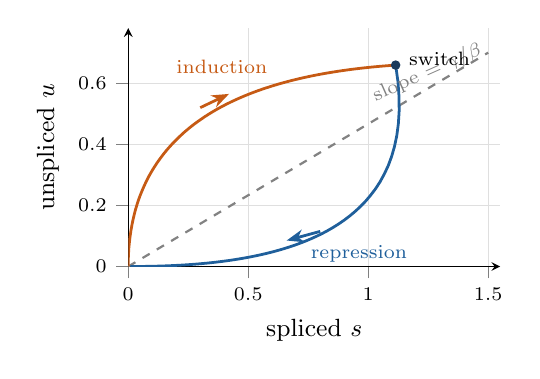
\begin{tikzpicture}
\begin{axis}[
  tarviaxis,
  xlabel={spliced $\spl$}, ylabel={unspliced $\uns$},
  xmin=0, xmax=1.55, ymin=0, ymax=0.78,
]
% steady-state diagonal, slope gamma/beta = 0.4667
\addplot[cGrey, dashed, line width=0.8pt, domain=0:1.5, samples=2]
  {0.4667*x};
% induction arm  (x = s(t), y = u(t))
\addplot[cU, domain=0:3, samples=140, variable=\t]
  ({1.4286*(1-exp(-0.7*\t)) - 1.25*(exp(-0.7*\t)-exp(-1.5*\t))},
   {0.6667*(1-exp(-1.5*\t))});
% repression arm
\addplot[cS, domain=0:8, samples=140, variable=\t]
  ({1.1143*exp(-0.7*\t) + 1.2362*(exp(-0.7*\t)-exp(-1.5*\t))},
   {0.6593*exp(-1.5*\t)});
% direction arrows
\draw[-{Stealth[length=2.2mm]}, cU, line width=1pt]
  (axis cs:0.30,0.52) -- (axis cs:0.42,0.565);
\draw[-{Stealth[length=2.2mm]}, cS, line width=1pt]
  (axis cs:0.80,0.115) -- (axis cs:0.66,0.085);
% annotations
\node[font=\scriptsize, cU, anchor=south east] at (axis cs:0.62,0.60) {induction};
\node[font=\scriptsize, cS, anchor=north west] at (axis cs:0.72,0.10) {repression};
\node[font=\scriptsize, cGrey, rotate=24, anchor=south] at (axis cs:1.28,0.575)
  {slope $=\gamma/\beta$};
\filldraw[tarvinavy] (axis cs:1.1143,0.6593) circle (1.5pt);
\node[font=\scriptsize, anchor=west] at (axis cs:1.13,0.68) {switch};
\end{axis}
\end{tikzpicture}
\caption{Two views of one gene, computed from the exact solutions
\eqref{eq:u-ind}--\eqref{eq:s-rep} with $\alpha = 1$, $\beta = 1.5$,
$\gamma = 0.7$, $\ts = 3$.
\textbf{Left:} time courses. Unspliced rises first and falls first; spliced
trails it, and continues rising briefly \emph{after} the gene has switched off.
That lag is the second term of \eqref{eq:s-ind}.
\textbf{Right:} the same trajectory drawn as $(\spl, \uns)$, which is what a
scatter over cells reveals. The lag turns the path into a counter-clockwise
loop; the induction arm sits above the steady-state diagonal and the repression
arm below it. The dashed diagonal has slope $\gamma/\beta$ by
\eqref{eq:ss-slope} and is the only feature of the data that identifies the
rates.}
\label{fig:dynamics}
\end{figure}

\subsection{A removable singularity at \texorpdfstring{$\gamma = \beta$}{gamma = beta}}

Both expressions for $\spl$ divide by $(\gamma - \beta)$. When a gene has
$\gamma \approx \beta$ the expression is numerically unstable, and at exact
equality it is undefined. Taking the limit $\gamma \to \beta$ in
\eqref{eq:s-ind} (write $\gamma = \beta + \varepsilon$ and expand to first
order in $\varepsilon$) gives the repeated-root solution
%
\begin{equation}
\spl(t) \;\xrightarrow[\gamma \to \beta]{}\;
\frac{\alpha}{\beta}\Big(1 - e^{-\beta t}\Big) - \alpha\, t\, e^{-\beta t},
\end{equation}
%
which is finite. The singularity is therefore removable. The implementation
does not branch on this case; it adds a small constant
($\texttt{eps} = 10^{-6}$) to the denominator, which is adequate in practice
since exact equality has measure zero.

%======================================================================
\section{What the data can and cannot tell us}
\label{sec:identifiability}
%======================================================================

A question that arises immediately on reading the model is: \emph{the splicing
and degradation rates were never measured, so how can we use them?} This
section answers that, and establishes two limitations that shape the rest of
the design.

\subsection{The rates are inferred, not measured}

$\beta$ and $\gamma$ are not experimental quantities supplied to the model.
They are \textbf{free parameters}, one per gene, declared as
\texttt{torch.nn.Parameter} and learned by gradient descent:
%
\begin{equation}
\beta_g = \operatorname{clamp}\big(\softplus(\theta^\beta_g),\, 0,\, 50\big),
\qquad
\gamma_g = \operatorname{clamp}\big(\softplus(\theta^\gamma_g),\, 0,\, 50\big).
\end{equation}
%
The softplus enforces positivity --- negative rates are physically meaningless
--- and the clamp keeps values in a range where the exponentials in
\eqref{eq:u-ind}--\eqref{eq:s-rep} do not overflow.

They are learned because the ODE solutions are the \emph{means of the
likelihood}. When observed $\uns$ and $\spl$ are scored against that likelihood
and the error is backpropagated, the gradient moves $\beta$ and $\gamma$
toward values that make the predicted curve pass through the observed data
cloud. This is ordinary maximum likelihood: an unmeasured quantity is
recovered from the pattern it leaves behind in quantities that \emph{were}
measured.

\subsection{What identifies them: the phase portrait}

Two features of the loop described in Section~\ref{sec:steady} carry
information about the rates:

\begin{center}
\begin{tabular}{@{}ll@{}}
\toprule
\textbf{Loop feature} & \textbf{What it determines} \\
\midrule
Slope of the steady-state diagonal & the ratio $\gamma/\beta$, via \eqref{eq:ss-slope} \\
Width / curvature of the loop & how \emph{different} $\beta$ and $\gamma$ are (the lag) \\
\bottomrule
\end{tabular}
\end{center}

A gene whose phase portrait is a shapeless blob carries \emph{no} information
about its own kinetics. This is the entire justification for the gene filter
described in Section~\ref{sec:gene-filter}.

\subsection{Scale invariance}

There is a fundamental limit on what can be recovered.

\begin{prop}[Scale non-identifiability]
\label{prop:scale}
For any $c > 0$, the reparameterisation
\[
\alpha \to c\alpha, \qquad \beta \to c\beta, \qquad \gamma \to c\gamma,
\qquad t \to t/c
\]
leaves $\uns(t)$ and $\spl(t)$ exactly unchanged.
\end{prop}

\begin{proof}
Substituting into \eqref{eq:u-ind},
\[
\frac{c\alpha}{c\beta}\Big(1 - e^{-c\beta \cdot t/c}\Big)
= \frac{\alpha}{\beta}\Big(1 - e^{-\beta t}\Big),
\]
and identically for \eqref{eq:s-ind}, since every rate appears either as a
ratio of two rates or multiplied by $t$. The same holds for the repression
branch.
\end{proof}

The data therefore cannot distinguish between a slow process observed over a
long interval and a fast process observed over a short one. Only \emph{ratios}
of rates are identifiable. Two consequences follow, and both are visible in
how results are reported.

\begin{keybox}
\textbf{Consequence 1: the time scale is a convention.}
The model fixes the remaining degree of freedom by setting
$\tmax = 20$ and initialising $\beta \approx 1$, so all rates are effectively
expressed in units of the splicing rate. Latent time is therefore in arbitrary
units, and only its \emph{ordering} is meaningful. This is why evaluation
reports Spearman correlation of pseudotime rather than absolute error.

\medskip
\textbf{Consequence 2: velocity magnitude is arbitrary, direction is not.}
Under the same rescaling $v \to c\,v$ by \eqref{eq:velocity}. The length of
every arrow is defined only up to one global constant, but its direction is
invariant. This is why every reported metric --- cross-boundary direction
accuracy, velocity confidence, cosine-based coherence --- is direction-based.
\end{keybox}

\subsection{What keeps the fit well behaved}

Because the problem is unidentifiable in general and non-convex in practice,
several components exist specifically to constrain it:

\begin{itemize}[leftmargin=*]
\item the \textbf{end penalty}, which forces the induction curve evaluated at
      the switch time to land on a data-derived anchor, pinning down where
      induction ends and thereby constraining $\gamma/\beta$;
\item the \textbf{sparse Dirichlet prior} on the state weights, which forces
      confident state assignment and blocks degenerate fits that hedge across
      all four states;
\item the \textbf{ODE residual loss}, which ties latent time to observed
      expression so that the rates cannot drift to compensate for a bad time
      estimate;
\item \textbf{data-driven initialisation} (Section~\ref{sec:init}), which
      places the optimiser in a sensible basin from the start.
\end{itemize}

%======================================================================
\section{Data preparation}
\label{sec:data}
%======================================================================

\subsection{Moments and scaling}

Three preprocessing steps precede training.

\begin{enumerate}[leftmargin=*]
\item \textbf{Moments.} First-order moments $M_s, M_u$ are computed upstream:
      each cell's counts are averaged over its $k$-nearest-neighbour
      neighbourhood. Raw droplet counts are far too sparse --- dominated by
      dropout zeros --- to fit a smooth ODE against.
\item \textbf{Min--max scaling} of $M_s$ and $M_u$ to $[0,1]$. This is
      required because the likelihood uses a Gaussian with a shared per-gene
      scale; without rescaling, highly expressed genes would dominate the
      reconstruction term entirely.
\item \textbf{Gene filtering}, described next.
\end{enumerate}

\subsection{The gene filter}
\label{sec:gene-filter}

A throwaway steady-state fit is run purely to compute a screening statistic:

\begin{lstlisting}
scv.tl.velocity(adata, mode="deterministic")
adata = adata[:, np.logical_and(adata.var.velocity_r2 > 0,
                                adata.var.velocity_gamma > 0)].copy()
adata = adata[:, adata.var.velocity_genes].copy()
\end{lstlisting}

The \texttt{deterministic} mode is the original steady-state estimator: for
each gene independently it fits a straight line $\uns \approx \gamma \spl$
through the extreme-quantile cells (those assumed to be at steady state, cf.
equation \eqref{eq:ss-slope}). Two quantities result per gene:
\texttt{velocity\_gamma}, the fitted slope, and \texttt{velocity\_r2}, the
coefficient of determination
%
\begin{equation}
R^2 = 1 - \frac{\mathrm{SS}_{\text{residual}}}{\mathrm{SS}_{\text{total}}}.
\end{equation}

The interpretation of the threshold is as follows:

\begin{center}
\begin{tabular}{@{}cl@{}}
\toprule
\textbf{Value} & \textbf{Meaning} \\
\midrule
$R^2 = 1$ & the line passes through every point exactly \\
$R^2 = 0$ & the line is no better than predicting the mean of $\uns$ \\
$R^2 < 0$ & the line is \emph{worse} than predicting the mean \\
\bottomrule
\end{tabular}
\end{center}

Negative $R^2$ is possible --- and is precisely what the filter targets ---
because the line is fitted on a \emph{subset} of cells (the extreme quantiles)
and then scored on \emph{all} cells. A gene with no coherent phase portrait
yields an arbitrarily placed line that scores worse than a flat mean. The
condition $R^2 > 0$ is thus a deliberately minimal bar: the steady-state line
must explain \emph{something}.

The companion condition $\gamma > 0$ rejects a negative fitted slope, which
would imply that unspliced and spliced counts anti-correlate --- impossible
under \eqref{eq:ode-s}, as it would require a negative degradation rate. The
third filter applies scVelo's own composite criterion, which additionally
requires sufficient detection across cells.

Retaining genes that fail these tests would cost twice over: model capacity is
spent fitting an ODE to noise, which given the non-convexity can drag the
optimiser into a poor basin; and because velocity direction is computed across
genes, uninformative genes dilute the signal in every cell's arrow.

\begin{keybox}
\textbf{A note on circularity.} This is a pre-filter that uses a simpler model
to select genes for a more complex one. The bar is deliberately permissive
($>0$, not $>0.5$) so that it removes genes carrying no signal rather than
selecting genes that happen to suit the steady-state model's assumptions.
\end{keybox}

\subsection{Initialisation}
\label{sec:init}

Because these ODEs admit many poor local optima, initialisation is
consequential. For each gene, the median over the top $1\%$ of cells by
unspliced count is taken, giving $(\uns_{\text{upper}}, \spl_{\text{upper}})$:
these cells sit near the top of induction, close to the steady state. They
supply three initial values:

\begin{center}
\begin{tabular}{@{}ll@{}}
\toprule
\textbf{Quantity} & \textbf{Initialisation} \\
\midrule
$\alpha$ & $\softplus^{-1}(\uns_{\text{upper}})$ \quad since $\uns^{*} = \alpha/\beta$ with $\beta \approx 1$ \\
switch anchor $(\uns_0, \spl_0)$ & $(\uns_{\text{upper}}, \spl_{\text{upper}})$ \\
$\gamma$ & $\uns_{\text{upper}} / \spl_{\text{upper}}$ \quad the steady-state slope, eq.~\eqref{eq:ss-slope} \\
$\beta$ & $\softplus(0.5) \approx 0.97$, i.e.\ effectively $1$ \\
\bottomrule
\end{tabular}
\end{center}

Setting $\beta \approx 1$ is the concrete act of fixing the scale degree of
freedom identified in Proposition~\ref{prop:scale}.

%======================================================================
\section{Model architecture}
\label{sec:architecture}
%======================================================================

\subsection{Why a variational autoencoder?}

The natural question is why a neural network is involved at all, when the
underlying model is a small ODE with a handful of parameters. The answer is a
parameter-counting argument.

Fitting the model requires, for every cell and every gene, a position in the
kinetic cycle: the induction progress $\rho$, the repression progress $\tau$,
and four state probabilities $\pi$. For $N = 3000$ cells and $G = 1000$ genes
that is on the order of $1.8 \times 10^7$ free parameters fitted against
$6 \times 10^6$ observations. The problem is hopelessly overparameterised, and
--- just as importantly --- every cell would be fitted in isolation, with no
sharing of information between similar cells.

\textbf{Amortised inference} replaces those per-cell parameters with a
\emph{function}. An encoder maps a cell's observed profile to a low-dimensional
state $z$; a decoder maps $z$ to the per-gene kinetic variables. The model then
carries roughly $10^5$ shared network weights instead of $10^7$ per-cell
parameters, and every cell's estimate is informed by every other cell because
all pass through the same weights.

\begin{figure}[htbp]
\centering
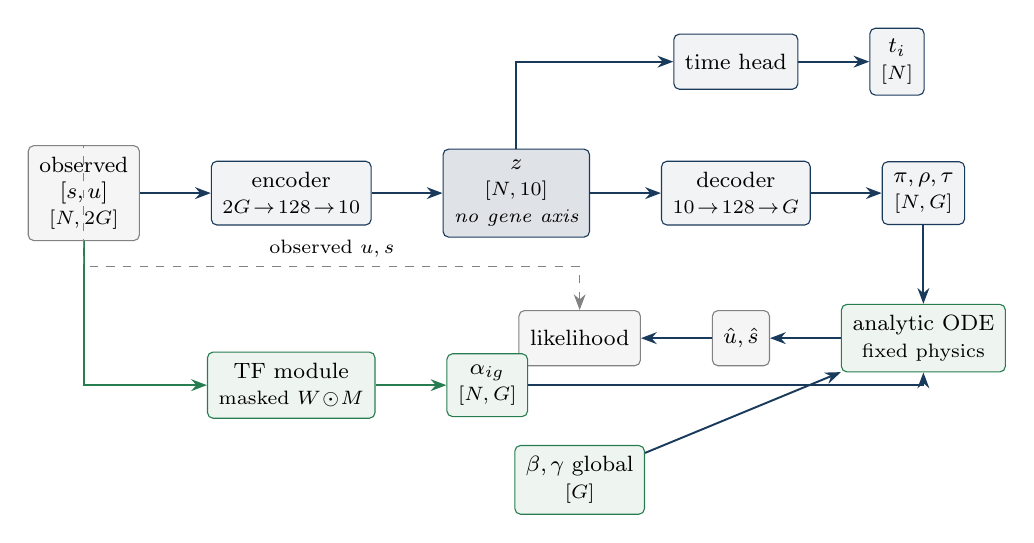
\begin{tikzpicture}[node distance=6mm and 9mm]

\node[dat] (data) {observed\\$[\spl,\uns]$\\{\scriptsize$[N,2G]$}};
\node[blk, right=of data] (enc) {encoder\\{\scriptsize$2G\!\to\!128\!\to\!10$}};
\node[blk, right=of enc, fill=tarvinavy!14] (z) {$z$\\{\scriptsize$[N,10]$}\\{\scriptsize\itshape no gene axis}};
\node[blk, right=of z] (dec) {decoder\\{\scriptsize$10\!\to\!128\!\to\!G$}};
\node[blk, right=of dec] (par) {$\pi,\rho,\tau$\\{\scriptsize$[N,G]$}};
\node[fix, below=10mm of par] (ode) {analytic ODE\\{\scriptsize fixed physics}};
\node[dat, left=of ode] (pred) {$\hat{\uns},\hat{\spl}$};
\node[dat, left=of pred] (lik) {likelihood};

% TF side channel
\node[blk, below=16mm of enc, fill=cGreen!8, draw=cGreen] (tf)
  {TF module\\{\scriptsize masked $W\!\odot\!M$}};
\node[blk, right=of tf, fill=cGreen!8, draw=cGreen] (alpha) {$\alpha_{ig}$\\{\scriptsize$[N,G]$}};

% time head
\node[blk, above=9mm of dec] (th) {time head};
\node[blk, right=of th] (ti) {$t_i$\\{\scriptsize$[N]$}};

% global params
\node[fix, below=10mm of lik] (rates) {$\beta,\gamma$ global\\{\scriptsize$[G]$}};

\draw[ar] (data) -- (enc);
\draw[ar] (enc)  -- (z);
\draw[ar] (z)    -- (dec);
\draw[ar] (dec)  -- (par);
\draw[ar] (par)  -- (ode);
\draw[ar] (ode)  -- (pred);
\draw[ar] (pred) -- (lik);
\draw[ar] (z)    |- (th);
\draw[ar] (th)   -- (ti);
\draw[ar] (alpha) -| (ode);
\draw[ar] (rates) -- (ode);
\draw[ar, draw=cGreen] (tf) -- (alpha);
\draw[ar, draw=cGreen] (data.south) |- ($(tf.west)+(-0.4,0)$) -- (tf.west);
\draw[{Stealth[length=2mm]}-, draw=cGrey, dashed]
  (lik.north) -- ++(0,0.55) -| node[pos=0.25, above, font=\scriptsize] {observed $\uns,\spl$} (data.north);
\end{tikzpicture}
\caption{Data flow. The encoder compresses the full expression profile into a
gene-free cell state $z$; the decoder re-creates the gene axis as kinetic
variables; the analytic ODE --- \emph{fixed physics, not learned} --- turns those
into predicted abundances that are scored against the observation. Two
quantities bypass the bottleneck: the global rates $\beta,\gamma$, and (in
green) the transcription rate $\alpha$, which is read directly from the
cell's own transcription-factor expression rather than from $z$.}
\label{fig:architecture}
\end{figure}

Note the final arrow. \textbf{The decoder does not predict expression.} It
predicts \emph{ODE parameters}, which then pass through the fixed analytic
solutions of Section~\ref{sec:kinetics}. The physics is imposed, not learned.
This is what keeps the model mechanistic and its outputs kinetically
interpretable, rather than a black-box autoencoder that happens to reconstruct
well.

Two further benefits follow from the choice of a \emph{variational}
autoencoder over a plain one. The KL term regularises the latent space to be
smooth and continuous, so nearby cells receive nearby codes; and because $z$ is
sampled rather than deterministic, repeated forward passes give a posterior
distribution over every downstream quantity, yielding uncertainty estimates
rather than point estimates.

\subsection{The encoder, and why \texorpdfstring{$z$}{z} is cell-level}
\label{sec:z-cell-level}

The encoder receives the concatenation of spliced and unspliced profiles and
returns a variational posterior:
%
\begin{equation}
q(z \mid \spl, \uns) = \mathcal{N}\big(\mu_z(\spl,\uns),\, \sigma_z^2(\spl,\uns)\big),
\qquad z \in \R^{10}.
\end{equation}

The claim that $z$ is a \emph{cell-level} quantity is not an interpretation but
a statement about tensor axes. Table~\ref{tab:axes} classifies every quantity
in the model.

\begin{table}[h]
\centering
\caption{Every quantity in TARVI, classified by the axes it carries.
$N$ = cells, $G$ = genes.}
\label{tab:axes}
\begin{tabular}{@{}llll@{}}
\toprule
\textbf{Quantity} & \textbf{Shape} & \textbf{Axes} & \textbf{Level} \\
\midrule
$\beta$, $\gamma$, $\ts$      & $[G]$        & gene only          & gene-level \\
$z$                            & $[N, 10]$    & cell only          & \textbf{cell-level} \\
\texttt{learned\_time}         & $[N]$        & cell only          & \textbf{cell-level} \\
$\rho$, $\tau$                 & $[N, G]$     & cell $\times$ gene & cell--gene \\
$\alpha$ (TF-regulated)        & $[N, G]$     & cell $\times$ gene & cell--gene \\
$\pi$                          & $[N, G, 4]$  & cell $\times$ gene $\times$ state & cell--gene \\
\bottomrule
\end{tabular}
\end{table}

$z$ has no gene axis. Tracing the computation makes clear why. The encoder's
first layer is dense, mapping $2G \to 128$: every gene connects to every hidden
unit and no per-gene pathway survives. The gene axis is destroyed on the first
matrix multiplication. Symmetrically, the decoder's layers map $10 \to 128 \to
G$: \emph{the gene axis is created there}, and does not exist upstream.

It is worth addressing the natural objection --- that $z$ is computed
\emph{from} gene expression and so ought to be gene-level. Being computed from
an axis is not the same as being indexed by it. A student's grade-point average
is computed from every course grade, but is a student-level quantity; ``the GPA
of Chemistry'' is a malformed question because the course axis was summed away.
Likewise ``the $z$ of gene \emph{Sox9}'' names no object. The ten coordinates of
$z$ are learned abstract factors --- position along a trajectory, lineage
branch, cell-cycle phase --- not gene slots.

Two structural pressures force $z$ to be a genuinely global summary. First, the
bottleneck: ten numbers cannot store per-gene information about a thousand
genes, so only what is shared across genes survives compression. Second, the
same $z$ must explain \emph{all} genes simultaneously through the decoder;
anything gene-specific would be useless to the other $G-1$ genes and is
squeezed out during training. This second pressure is exactly what couples the
genes together and yields a coherent cell-level trajectory rather than $G$
independent gene clocks.

\subsection{The decoder and the four kinetic states}

The decoder maps $z$ to three per-cell, per-gene quantities:

\begin{center}
\begin{tabular}{@{}lll@{}}
\toprule
\textbf{Output} & \textbf{Shape} & \textbf{Meaning} \\
\midrule
$\pi_\alpha$ & $[N, G, 4]$ & Dirichlet concentrations over kinetic states \\
$\rho$  & $[N, G] \in (0,1)$ & fractional progress through induction \\
$\tau$  & $[N, G] \in (0,1)$ & fractional progress through repression \\
\bottomrule
\end{tabular}
\end{center}

\subsubsection{Two trunks and three heads}

Structurally the decoder is a pair of independent multilayer trunks, each
reading $z$, followed by three output heads:

\begin{lstlisting}
# two independent trunks, both reading z
self.rho_first_decoder = FCLayers(n_in=10, n_out=128)   # serves rho and tau
self.pi_first_decoder  = FCLayers(n_in=10, n_out=128)   # serves pi

# three output heads
self.px_rho_decoder = nn.Sequential(nn.Linear(128, G), nn.Sigmoid())
self.px_tau_decoder = nn.Sequential(nn.Linear(128, G), nn.Sigmoid())
self.px_pi_decoder  = nn.Linear(128, 4 * G)
\end{lstlisting}

Here \texttt{FCLayers} is the scvi-tools block --- Linear, batch norm, layer
norm, ReLU and dropout. The progress variables $\rho$ and $\tau$ share a trunk,
since both describe a position within a phase and can reuse the same features,
but receive separate heads because they describe \emph{different} phases. The
state weights are given their own trunk entirely.

\begin{figure}[htbp]
\centering
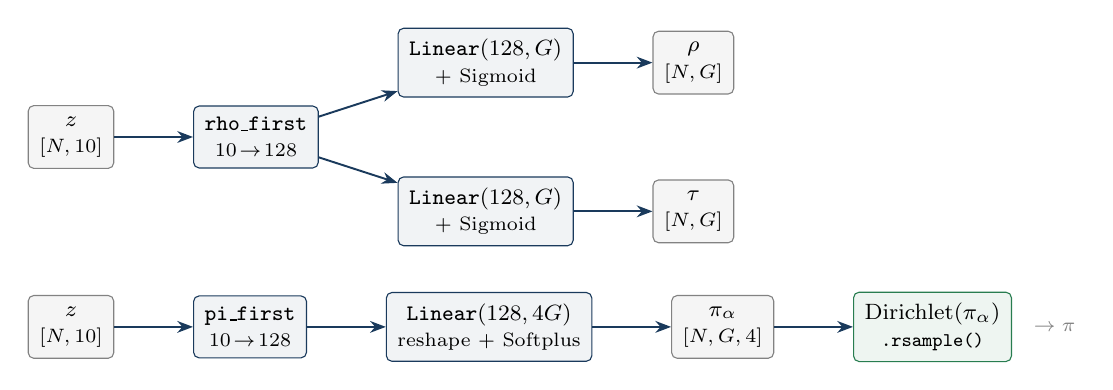
\begin{tikzpicture}[node distance=5mm and 10mm]
\node[dat] (z1) {$z$\\{\scriptsize$[N,10]$}};
\node[blk, right=of z1] (rt) {\texttt{rho\_first}\\{\scriptsize$10\!\to\!128$}};
\node[blk, above right=1mm and 10mm of rt] (rh) {\texttt{Linear}$(128,G)$\\{\scriptsize$+$ Sigmoid}};
\node[blk, below right=1mm and 10mm of rt] (th) {\texttt{Linear}$(128,G)$\\{\scriptsize$+$ Sigmoid}};
\node[dat, right=of rh] (rho) {$\rho$\\{\scriptsize$[N,G]$}};
\node[dat, right=of th] (tau) {$\tau$\\{\scriptsize$[N,G]$}};

\node[dat, below=16mm of z1] (z2) {$z$\\{\scriptsize$[N,10]$}};
\node[blk, right=of z2] (pt) {\texttt{pi\_first}\\{\scriptsize$10\!\to\!128$}};
\node[blk, right=of pt] (ph) {\texttt{Linear}$(128,4G)$\\{\scriptsize reshape $+$ Softplus}};
\node[dat, right=of ph] (pia) {$\pi_\alpha$\\{\scriptsize$[N,G,4]$}};
\node[fix, right=of pia] (pi) {$\mathrm{Dirichlet}(\pi_\alpha)$\\{\scriptsize\texttt{.rsample()}}};

\draw[ar] (z1) -- (rt);
\draw[ar] (rt) -- (rh);
\draw[ar] (rt) -- (th);
\draw[ar] (rh) -- (rho);
\draw[ar] (th) -- (tau);
\draw[ar] (z2) -- (pt);
\draw[ar] (pt) -- (ph);
\draw[ar] (ph) -- (pia);
\draw[ar] (pia) -- (pi);
\node[font=\scriptsize, cGrey, anchor=west] at ($(pi.east)+(0.15,0)$) {$\to \pi$};
\end{tikzpicture}
\caption{Decoder structure. Two trunks map the ten-dimensional cell state to
128-dimensional hidden vectors --- still with no gene axis. The output heads
create the gene axis, each of the $G$ output units being a distinct learned
readout of the same shared hidden vector.}
\label{fig:decoder}
\end{figure}

\subsubsection{Where the gene axis is created}

This is the mechanical counterpart to Section~\ref{sec:z-cell-level}. The trunks
emit a 128-dimensional vector \emph{per cell}; there are still no genes. The
gene axis is manufactured by the output layers,
%
\begin{equation}
\underbrace{h_\rho \in \R^{128}}_{\text{per cell}}
\;\xrightarrow{\;W \in \R^{G \times 128}\;}\;
\underbrace{\rho \in \R^{G}}_{\text{per cell, per gene}} ,
\end{equation}
%
in which each of the $G$ output units is a different learned linear readout of
the same shared hidden vector. Gene $g$'s row of $W$ poses its own question of
the cell state. This is how a single ten-dimensional code can specify positions
for a thousand genes: the genes differ in \emph{how they read} the cell state,
not in what state information reaches them.

\subsubsection{Why sigmoid on \texorpdfstring{$\rho$}{rho} and \texorpdfstring{$\tau$}{tau}}

Neither variable is a time. Both are \emph{fractions of a phase}, converted to
times by scaling:
%
\begin{equation}
t_{\text{ind}} = \ts \cdot \rho \in (0, \ts),
\qquad
t_{\text{rep}} = (\tmax - \ts)\cdot \tau \in (0, \tmax - \ts).
\end{equation}

This is a parameterisation device rather than a cosmetic choice. The
alternative --- predicting an absolute time and hoping it falls inside the
correct phase --- would require a penalty term and could still be violated. Here
the constraint is \emph{structural}: the sigmoid bounds the output to $(0,1)$,
and multiplying by the phase width makes it arithmetically impossible for an
induction time to exceed the switch point. No loss term is needed and no
invalid state is reachable.

A second consequence is that $\rho$ and $\tau$ are \emph{relative} coordinates.
A cell with $\rho = 0.5$ is halfway through induction \emph{for that gene},
whether that gene's switch time is $2$ or $18$.

\subsubsection{Why softplus on \texorpdfstring{$\pi$}{pi}: concentrations are not probabilities}

The decoder does not emit probabilities. It emits Dirichlet
\emph{concentrations}, which are positive and unnormalised; the probabilities
appear one step later, by sampling:

\begin{lstlisting}
px_pi_alpha = Softplus(reshape(px_pi_decoder(h_pi), (N, G, 4)))  # decoder output
px_pi       = Dirichlet(px_pi_alpha).rsample()                   # what is used
\end{lstlisting}

Softplus enforces positivity, which is the Dirichlet's only requirement on its
parameters. The distinction between the two objects matters:

\begin{center}
\begin{tabular}{@{}lllp{5.6cm}@{}}
\toprule
& \textbf{Shape} & \textbf{Constraint} & \textbf{Meaning} \\
\midrule
$\pi_\alpha$ (decoder output) & $[N,G,4]$ & $>0$ & concentrations: both the preferred state \emph{and} the confidence \\
$\pi$ (after \texttt{rsample}) & $[N,G,4]$ & sums to $1$ & the state weights entering the mixture \\
\bottomrule
\end{tabular}
\end{center}

Two things follow. First, \textbf{confidence is represented separately from
preference}: the concentrations $(10,1,1,1)$ and $(1.0,0.1,0.1,0.1)$ induce the
same mean probabilities but very different certainty, a distinction a plain
softmax cannot express since it retains only the ratio. Second,
\texttt{rsample} is the \emph{reparameterised} Dirichlet draw, so gradients pass
through the state assignment. Sampling is ordinarily a barrier to
backpropagation; here it is not, which is why no \texttt{argmax} appears
anywhere in the model --- the state assignment remains a differentiable mixture
throughout.

\subsubsection{What the decoder deliberately does not produce}

\begin{center}
\begin{tabular}{@{}llp{6.4cm}@{}}
\toprule
\textbf{Quantity} & \textbf{Source} & \textbf{Why not the decoder} \\
\midrule
$\beta$, $\gamma$ & global parameters $[G]$ & properties of the gene, not of the cell; no cell axis is required \\
$\alpha$ & TF module, read from data & requires specific TF identity, which cannot survive the ten-dimensional bottleneck \\
$\ts$ & global parameter $[G]$ & a property of the gene's kinetics, shared by all cells \\
\bottomrule
\end{tabular}
\end{center}

\begin{keybox}
The division of labour is therefore clean: \textbf{the decoder answers
\emph{where} a cell sits in each gene's cycle; the rate parameters answer
\emph{how fast} that cycle runs.}
\end{keybox}

\paragraph{A subtlety in the implementation.} The two trunks are not fed
identically:
%
\begin{lstlisting}
rho_first = self.rho_first_decoder(z_in)   # z_in - may be masked
pi_first  = self.pi_first_decoder(z)       # z    - always full
\end{lstlisting}
%
Here \texttt{z\_in} is the latent-dimension-masked variant used by the
interpretability path, which restricts the decoder to a single latent dimension
in order to ask what that dimension encodes. The masking therefore applies to
$\rho$ and $\tau$ but not to $\pi$. This is harmless during ordinary training,
where the two are identical, but is worth knowing before running per-dimension
attribution: the state assignment will not respond to the mask.

\subsubsection{The four states}

Writing $\ts$ for the learned per-gene switch time, the four states and their
times are:

\begin{center}
\begin{tabular}{@{}lll@{}}
\toprule
\textbf{State} & \textbf{Time} & \textbf{Predicted $(\uns, \spl)$} \\
\midrule
Induction         & $t = \ts\,\rho$                & eqs.\ \eqref{eq:u-ind}, \eqref{eq:s-ind} \\
Induction steady  & ---                            & $(\alpha/\beta,\ \alpha/\gamma)$ \\
Repression        & $t = (\tmax - \ts)\,\tau$      & eqs.\ \eqref{eq:u-rep}, \eqref{eq:s-rep} \\
Repression steady & ---                            & $(0, 0)$ \\
\bottomrule
\end{tabular}
\end{center}

Each state contributes a Gaussian centred on its predicted $(\uns, \spl)$ with a
learned per-gene scale; these are combined by \texttt{MixtureSameFamily}
weighted by the sampled $\pi$. The repression-steady component receives a scale
reduced by a factor of ten, since it is an exact point rather than a fitted
curve.

\subsection{Contribution 1: TF-regulated transcription}

\subsubsection{Building the prior}

A binary mask of known regulatory relationships is assembled from ENCODE
ChIP-seq and ChEA 2016. TF--target pairs are parsed from both sources, gene
names are resolved case-insensitively against the dataset so that only TFs and
targets actually present survive, evidence is counted per pair, and the top 99
TFs per target gene are retained. The result is a mask
$M \in \{0,1\}^{G \times T}$ together with initial weights given by the
Spearman correlation between each TF's and target's expression, computed over
cells where both exceed a small threshold and scaled by $0.1$.

\subsubsection{The cell-specific rate}

The transcription rate is then computed per cell:
%
\begin{keybox}
\begin{equation}
\alpha_{ig} = \operatorname{clamp}\Big(
\softplus\Big(\textstyle\sum_{k} \big(w_{gk} \odot M_{gk}\big)\, \mathrm{TF}_k(i) + b_g\Big),
\; 0,\; 50 \Big)
\label{eq:tf-alpha}
\end{equation}
\end{keybox}
%
where $b_g$ is a learnable basal rate warm-started from the static per-gene
$\alpha$, and $\mathrm{TF}_k(i)$ is the spliced expression of the $k$-th
transcription factor in cell $i$, read directly from the data rather than from
$z$.

Three points are worth emphasising. The mask is applied \emph{inside} the
forward pass, so gradients for non-edges are structurally zero and the model
cannot invent regulation --- it learns only the strength and sign of edges that
ChIP-seq evidence already supports. The static $\alpha$ is frozen when TF
regulation is active, so there is no competing pathway. And a mild $L_1$
penalty on $W$ ensures each gene ends up driven by a few dominant regulators
rather than all 99, which makes the fitted $W$ readable as a regulatory
network.

Comparing with the baseline: where VeloVI has $\alpha_g$, a single number per
gene shared by all cells, TARVI has $\alpha_{ig}$, an $[N \times G]$ matrix
that varies across the manifold according to which transcription factors each
cell expresses.

\subsubsection{How \texorpdfstring{$\alpha$}{alpha} enters the ODE}
\label{sec:alpha-in-ode}

The transcription rate appears in exactly three places, and in every one of
them it appears as a \emph{multiplicative factor}:

\begin{center}
\begin{tabular}{@{}ll@{}}
\toprule
\textbf{Location} & \textbf{Role of $\alpha$} \\
\midrule
Induction curve, eqs.\ \eqref{eq:u-ind}, \eqref{eq:s-ind} & overall amplitude \\
Induction steady state & the plateau $(\alpha/\beta,\ \alpha/\gamma)$ \\
Repression, eqs.\ \eqref{eq:u-rep}, \eqref{eq:s-rep} & only via $(\uns_0, \spl_0)$, since $\alpha = 0$ there \\
\bottomrule
\end{tabular}
\end{center}

This is clearest when the induction solution is factored:
%
\begin{equation}
\uns(t) = \alpha \cdot \underbrace{\tfrac{1}{\beta}\big(1 - e^{-\beta t}\big)}_{\text{shape --- independent of }\alpha} .
\end{equation}
%
\textbf{$\alpha$ sets the height of the curve; $\beta$ and $\gamma$ set its
shape; $t$ sets the position along it.} These are three separate roles, and the
distinction is what the next subsection turns on.

\subsubsection{Velocity is directly proportional to \texorpdfstring{$\alpha$}{alpha}}

Substituting the induction solutions into $v = \beta \uns - \gamma \spl$, the
terms collapse. With
$\beta \uns = \alpha(1 - e^{-\beta t})$ and
$\gamma \spl = \alpha(1-e^{-\gamma t}) + \frac{\alpha\gamma}{\gamma-\beta}(e^{-\gamma t} - e^{-\beta t})$,
%
\begin{align}
v_{\text{ind}}
&= \alpha\big(e^{-\gamma t} - e^{-\beta t}\big)\Big[1 - \tfrac{\gamma}{\gamma-\beta}\Big]
 = \alpha\big(e^{-\gamma t} - e^{-\beta t}\big)\Big[\tfrac{-\beta}{\gamma-\beta}\Big],
\end{align}
%
that is,
%
\begin{keybox}
\begin{equation}
\boxed{\; v_{\text{ind}}(t) = \frac{\alpha\beta}{\gamma - \beta}
\Big(e^{-\beta t} - e^{-\gamma t}\Big) \;}
\label{eq:v-prop-alpha}
\end{equation}
\emph{Induction velocity is exactly proportional to the transcription rate.}
\end{keybox}
%
The expression vanishes at $t = 0$ and again as $t \to \infty$, peaking in
between --- correct for a gene that ramps up and then plateaus. The point of
\eqref{eq:v-prop-alpha} is that $\alpha$ is not a peripheral nuisance
parameter: it is the \emph{amplitude of the velocity itself}. Doubling a cell's
transcription rate exactly doubles its velocity for that gene at a fixed time.

\subsubsection{Why a cell-specific \texorpdfstring{$\alpha$}{alpha} helps}

\paragraph{It separates amplitude from time.} With one $\alpha$ per gene, every
cell lies on a \emph{single shared curve}. The only mechanism available to
explain a cell with high expression is that it has progressed further through
induction. Genuine differences in regulatory drive are therefore silently
re-encoded as differences in developmental time.

Figure~\ref{fig:alpha} makes the consequence concrete. Two cells are observed
at the identical value $\uns = 0.5$, but one has strong transcription-factor
support and the other weak. Under \eqref{eq:ode-u} their instantaneous
dynamics differ by a factor of fifteen:
%
\begin{center}
\begin{tabular}{@{}lcccc@{}}
\toprule
& TF activity & $\alpha$ & inferred $t$ & $d\uns/dt = \alpha - \beta \uns$ \\
\midrule
Cell A & high & $2.0$ & $0.29$ & $\mathbf{1.5}$ \\
Cell B & low  & $0.6$ & $1.79$ & $\mathbf{0.1}$ \\
\bottomrule
\end{tabular}
\end{center}
%
A static-$\alpha$ model must assign these two cells the same time \emph{and}
the same velocity. It has no vocabulary for ``these cells differ in regulatory
drive rather than in developmental stage''.

\begin{figure}[htbp]
\centering
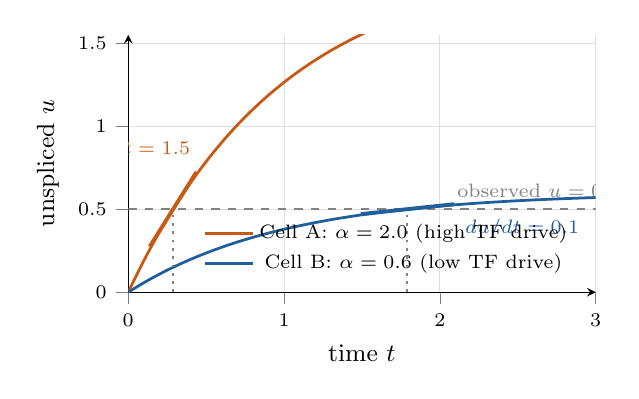
\begin{tikzpicture}
\begin{axis}[
  tarviaxis, width=0.62\textwidth, height=0.40\textwidth,
  xlabel={time $t$}, ylabel={unspliced $\uns$},
  xmin=0, xmax=3, ymin=0, ymax=1.55,
  legend pos=south east,
]
\addplot[cU, domain=0:3, samples=120] {2.0*(1-exp(-x))};
\addlegendentry{Cell A: $\alpha = 2.0$ (high TF drive)}
\addplot[cS, domain=0:3, samples=120] {0.6*(1-exp(-x))};
\addlegendentry{Cell B: $\alpha = 0.6$ (low TF drive)}
% observed level
\addplot[cGrey, dashed, line width=0.8pt, forget plot]
  coordinates {(0,0.5) (3,0.5)};
\node[font=\scriptsize, cGrey, anchor=south west] at (axis cs:2.05,0.51)
  {observed $\uns = 0.5$};
% drop lines
\addplot[cGrey, dotted, line width=0.7pt, forget plot]
  coordinates {(0.288,0) (0.288,0.5)};
\addplot[cGrey, dotted, line width=0.7pt, forget plot]
  coordinates {(1.792,0) (1.792,0.5)};
% tangents showing du/dt
\draw[cU, line width=1.4pt] (axis cs:0.138,0.275) -- (axis cs:0.438,0.725);
\draw[cS, line width=1.4pt] (axis cs:1.492,0.470) -- (axis cs:2.092,0.530);
\node[font=\scriptsize, cU, anchor=south east] at (axis cs:0.46,0.74)
  {$d\uns/dt = 1.5$};
\node[font=\scriptsize, cS, anchor=north west] at (axis cs:2.10,0.50)
  {$d\uns/dt = 0.1$};
\node[font=\scriptsize, anchor=north] at (axis cs:0.288,-0.03) {$t_A$};
\node[font=\scriptsize, anchor=north] at (axis cs:1.792,-0.03) {$t_B$};
\end{axis}
\end{tikzpicture}
\caption{Why a cell-specific $\alpha$ matters. Both cells are measured at
$\uns = 0.5$, but $\alpha$ scales the whole induction curve, so the same
observation places them at very different points in the cycle: cell A is early
on a tall curve and still climbing steeply, cell B is near the ceiling of a
short curve and has almost stopped. The heavy segments are the tangents, whose
slopes are the unspliced velocities --- a factor of fifteen apart. A model with
one $\alpha$ per gene has a single curve and must give both cells the same
answer.}
\label{fig:alpha}
\end{figure}

\paragraph{It costs almost no parameters.} A freely fitted $\alpha_{ig}$ would
introduce $N \times G$ parameters --- entirely unidentifiable, capable of
fitting any data exactly and therefore explaining nothing. Instead
$\alpha_{ig}$ varies over all $N \times G$ entries while being \emph{generated}
by only $|M| + G$ parameters (the non-zero mask weights plus the basal rates),
shared across every cell. The cell-to-cell variation is supplied by
\emph{measured transcription-factor expression}, not by free parameters:
cell-specificity is bought with data rather than with degrees of freedom.

\paragraph{It is a second channel that bypasses the bottleneck.} As established
in Section~\ref{sec:z-cell-level}, $z$ has ten dimensions and therefore
necessarily destroys gene-specific detail. The TF pathway reads transcription
factor expression \emph{directly from the data}, not through $z$ --- the green
route in Figure~\ref{fig:architecture}. Specific regulatory identity, of the
form ``this particular cell strongly expresses this particular factor'',
therefore reaches $\alpha$ even though it could never survive compression into
ten dimensions.

\paragraph{It yields a readable network.} After training, $W \odot M$ is a
gene-by-TF matrix of learned regulatory strengths with signs, sparsified by the
$L_1$ penalty. This is a scientific output --- an inferred regulatory network
--- obtained as a by-product of velocity estimation.

\begin{keybox}
\textbf{A note on attribution.} The mechanism above is the design rationale for
a cell-specific $\alpha$. The component ablation, however, attributes most of
the \emph{pseudotime} improvement to the ODE residual loss and to
velocity--pseudotime blending, with TF regulation contributing principally on
the interpretability side. Both statements should be made; claiming the
headline metric for this component would overstate what the ablation supports.
\end{keybox}

\subsection{The latent time head}
\label{sec:time-head}

A small residual network maps the cell state to a scalar time:
%
\begin{align}
h &= \mathrm{ReLU}(W_1 z) + W_{\text{skip}}\, z, \\
h &= \mathrm{ReLU}\big(W_2\,\mathrm{LayerNorm}(h)\big), \\
t_i &= \sigma(W_{\text{out}} h) \in [0,1].
\end{align}

\subsubsection{Why the input is \texorpdfstring{$z$}{z}}

Latent time must be one number per cell, and by Table~\ref{tab:axes} the only
cell-indexed, gene-free representation available is $z$. Beyond that necessity,
reading from $z$ has four advantages: the head sees the \emph{same} cell state
that generates the kinetics, so time and the ODE parameters cannot disagree
about what cell this is; $z$ is already denoised by the encoder, so pseudotime
does not inherit dropout noise; the KL term makes $z$ continuous, so nearby
cells automatically receive nearby times; and a $10 \to 1$ regression is
learnable from a few thousand cells, where $2G \to 1$ would not be.

There is also a less obvious effect. Because the ODE residual loss
(Section~\ref{sec:loss-b}) reaches the head, and the head's input is $z$, the
gradient continues into the encoder:
%
\begin{equation}
\mathcal{L}_{\text{res}} \;\to\; t_i \;\to\; \text{time head} \;\to\; z \;\to\; \text{encoder}.
\end{equation}
%
The supervision therefore \emph{reshapes the latent space itself} to be
temporally organised. This is a substantial part of why pseudotime improves,
and it is the reason the companion loss detaches its \emph{target} but not its
prediction.

\subsubsection{The skip connection}
\label{sec:skip}

Rather than a single chain of layers, the cell state travels two routes which
are then summed:

\begin{figure}[htbp]
\centering
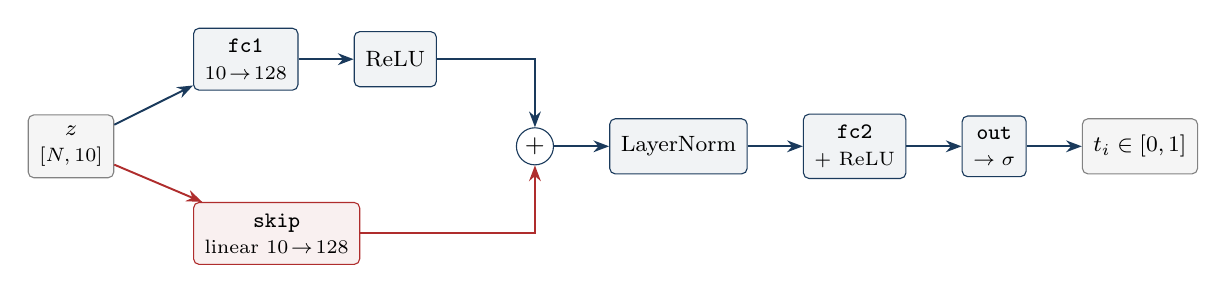
\begin{tikzpicture}[node distance=5mm and 7mm]
\node[dat] (z) {$z$\\{\scriptsize$[N,10]$}};
\node[blk, above right=3mm and 10mm of z] (fc1) {\texttt{fc1}\\{\scriptsize$10\!\to\!128$}};
\node[blk, right=of fc1] (relu) {ReLU};
\node[blk, below right=3mm and 10mm of z, draw=cRed, fill=cRed!7] (skip)
  {\texttt{skip}\\{\scriptsize linear $10\!\to\!128$}};
\node[circle, draw=tarvinavy, inner sep=1.4pt, font=\small,
      right=17mm of z, xshift=34mm] (plus) {$+$};
\node[blk, right=of plus] (ln) {LayerNorm};
\node[blk, right=of ln] (fc2) {\texttt{fc2}\\{\scriptsize$+$ ReLU}};
\node[blk, right=of fc2] (out) {\texttt{out}\\{\scriptsize$\to\sigma$}};
\node[dat, right=of out] (t) {$t_i \in [0,1]$};

\draw[ar] (z) -- (fc1);
\draw[ar] (fc1) -- (relu);
\draw[ar] (relu) -| (plus);
\draw[ar, draw=cRed] (z) -- (skip);
\draw[ar, draw=cRed] (skip) -| (plus);
\draw[ar] (plus) -- (ln);
\draw[ar] (ln) -- (fc2);
\draw[ar] (fc2) -- (out);
\draw[ar] (out) -- (t);
\end{tikzpicture}
\caption{The time head. The upper branch passes through the nonlinearity; the
lower branch (red) bypasses it with a plain linear map. Because their
dimensions differ, the shortcut cannot be the identity and must itself be a
learned projection.}
\label{fig:skip}
\end{figure}

The lower branch bypasses the nonlinearity entirely. That is the defining idea
of a skip (or \emph{residual}) connection: information is given a shortcut
around one or more layers instead of being forced through them.

Two variants exist. The classical form introduced with residual networks is
$h = f(x) + x$, a literal identity shortcut, available only when input and
output dimensions agree. Here they do not --- $\R^{10}$ against $\R^{128}$ ---
so a learned linear map stands in its place, $h = f(x) + W_{\text{skip}}x$. This
is termed a \emph{projection shortcut}.

The effect on the computation is small to write down but consequential:

\begin{center}
\begin{tabular}{@{}ll@{}}
\toprule
\textbf{Without skip} & $h = \mathrm{ReLU}(W_1 z)$ \\
\textbf{With skip}    & $h = \mathrm{ReLU}(W_1 z) + W_{\text{skip}}\, z$ \\
\bottomrule
\end{tabular}
\end{center}

The term $\mathrm{ReLU}(W_1 z)$ is non-negative and \emph{exactly zero} on half
of its input space. Adding $W_{\text{skip}} z$ contributes a plain linear
component that is always active. The head therefore computes a linear function
of $z$ plus a nonlinear correction, rather than having to construct everything
out of rectified pieces.

\begin{keybox}
\textbf{The question is not one of representational capacity.} A plain
multilayer perceptron is a universal approximator: $10 \to 128 \to 128 \to 1$
with rectified units can represent any smooth function of $z$, a linear one
included. The skip therefore buys no expressiveness. What it buys is
\emph{what is easy to learn from a random initialisation}, and \emph{what
happens when training goes wrong}.
\end{keybox}

\paragraph{It encodes the right prior.} Pseudotime is approximately linear in
$z$: in a well-trained VAE the trajectory tends to lie along a principal
direction of the latent space, so the ideal map is close to a linear ramp with
corrections where the trajectory bends. Suppose that ideal map is
$t \approx w^{\!\top} z$. The two architectures then face quite different
learning problems:

\begin{center}
\begin{tabular}{@{}ll@{}}
\toprule
\textbf{Without skip} & the weights must construct $w^{\!\top} z$ from scratch out of rectified pieces \\
\textbf{With skip}    & $W_{\text{skip}}$ \emph{is} the linear part; $W_1$ learns only the deviation \\
\bottomrule
\end{tabular}
\end{center}

Both reach the same final capacity, but by very different optimisation paths:
the second starts near a sensible answer and refines it, whereas the first must
first discover the linear structure before it can refine anything.

\paragraph{The failure mode here is ties, not error.} Without the skip a ReLU
network must \emph{approximate} a straight line using piecewise-linear
segments, which with a finite number of active pieces produces a staircase:
flat plateaus joined by steps. This deserves emphasis because of how it
interacts with the evaluation metric.

\begin{keybox}
A staircase approximation to a ramp has \emph{small squared error} --- it is
never far from the correct value --- yet every flat segment assigns an identical
time to many cells, and so destroys the ordering information within it. Since
pseudotime is scored by Spearman correlation, a rank statistic, the consequence
is that \textbf{the training loss can look perfectly healthy while the reported
metric collapses.} The linear bypass removes the staircase by construction,
because a genuinely linear component always varies continuously with $z$.
\end{keybox}

\paragraph{It guarantees a gradient path.} Differentiating the two branches,
%
\begin{equation}
\frac{\partial h}{\partial z}
= \underbrace{\mathrm{ReLU}'(W_1 z)\, W_1}_{\text{zero wherever units are dead}}
\;+\; \underbrace{W_{\text{skip}}}_{\text{always nonzero}} .
\end{equation}
%
A rectified unit with negative pre-activation passes exactly zero gradient, and
if enough units die the gradient reaching $z$ collapses. This matters more here
than in a typical network: as established in Section~\ref{sec:time-head}, the
time head is the only conduit through which the ODE residual loss reaches $z$
and reorganises the latent space. Were the head to close that path, nothing
would raise an error --- the pseudotime would simply, and silently, get worse.

\paragraph{It keeps the output sigmoid responsive.} The final activation is
$\sigma(\cdot)$, whose derivative vanishes at both extremes. If pre-activations
drift large the gradient dies and every cell collapses to $t \approx 0$ or
$t \approx 1$ --- a genuine risk when several losses push simultaneously on one
small head. This is also why the LayerNorm is placed \emph{after} the addition
rather than before it: summing two branches yields an output of unpredictable
scale, and either branch could dominate the other by magnitude alone.
Normalising the combined signal re-standardises it and holds the sigmoid in its
responsive region.

\paragraph{Is it strictly necessary?} No. A plain two-layer perceptron would in
all likelihood train to something reasonable, and it would be an overstatement
to claim the model fails without the shortcut.

The trade, however, is markedly lopsided. The skip costs a single
$10 \times 128$ matrix --- 1{,}280 parameters, negligible beside the rest of the
model --- and in exchange it protects a component whose failure is
\emph{silent} (Section~\ref{sec:time-head}: the head is the sole route by which
the ODE residual loss reaches $z$) and whose downstream influence is large.
That asymmetry is what justifies it: not evidence that the shortcut is
required, but the observation that it is nearly free and closes a failure mode
the training loss would not have revealed.

%======================================================================
\section{Training without ground truth}
\label{sec:training}
%======================================================================

\subsection{The principle}

No ground-truth velocity, latent time, or kinetic rate is available for any
dataset. This appears to make a loss function impossible: a loss compares an
answer to a correct answer, and there is no correct answer to compare against.

The resolution is that \textbf{velocity is never optimised}. What is optimised
is the reconstruction of the observed data:

\begin{lstlisting}
reconst_loss_s = -mixture_dist_s.log_prob(spliced)     # target = observed s
reconst_loss_u = -mixture_dist_u.log_prob(unspliced)   # target = observed u
\end{lstlisting}

The model proposes rates and times; the ODE converts these into predicted
$\hat{\uns}, \hat{\spl}$; those predictions are scored against what was actually
measured. The observed counts \emph{are} the ground truth. ``Unsupervised''
here means \emph{no external labels}, not \emph{no target}.

Velocity then follows for free, because by \eqref{eq:velocity} it is a
deterministic function of quantities the reconstruction has already pinned
down. The same applies to latent time, state assignment, and the TF weights:
all are \emph{latent variables inferred as a by-product} of explaining the
data. A quantity that is never directly optimised needs no label.

\begin{keybox}
\textbf{The bathtub picture.} Two connected tanks: a tap fills the first at
rate $\alpha$, a pipe drains it into the second at rate $\beta$, and a drain
empties the second at rate $\gamma$. The taps are hidden; only the water levels
are visible. The model guesses tap settings, predicts the resulting levels, and
is corrected by the discrepancy against the measured levels. Velocity --- is
the second tank filling or draining --- is then simple arithmetic on the
recovered taps.
\end{keybox}

\subsection{A worked example}

Consider one cell and one gene. Suppose the measured values are
$\uns = 0.80$ and $\spl = 0.30$.

\paragraph{Round 1.} The model's current guess is $\alpha = 1$, $\beta = 1$,
$\gamma = 2$, with this cell at $t = 0.5$ in the induction state. Substituting
into \eqref{eq:u-ind} and \eqref{eq:s-ind}:
%
\begin{align}
\hat{\uns} &= \tfrac{1}{1}\big(1 - e^{-0.5}\big) = 0.39, \\
\hat{\spl} &= \tfrac{1}{2}\big(1 - e^{-1}\big) + \tfrac{1}{2-1}\big(e^{-1} - e^{-0.5}\big) = 0.08.
\end{align}

\begin{center}
\begin{tabular}{@{}lccc@{}}
\toprule
 & predicted & measured & error \\
\midrule
$\uns$ & $0.39$ & $0.80$ & $-0.41$ \\
$\spl$ & $0.08$ & $0.30$ & $-0.22$ \\
\midrule
\multicolumn{3}{r}{squared error} & $\mathbf{0.21}$ \\
\bottomrule
\end{tabular}
\end{center}

Both predictions are too low, so the gradient increases $\alpha$.

\paragraph{Round 2.} With $\alpha = 2$ and the other parameters unchanged:
%
\begin{equation}
\hat{\uns} = 0.79, \qquad \hat{\spl} = 0.15.
\end{equation}

\begin{center}
\begin{tabular}{@{}lccc@{}}
\toprule
 & predicted & measured & error \\
\midrule
$\uns$ & $0.79$ & $0.80$ & $-0.01$ \\
$\spl$ & $0.15$ & $0.30$ & $-0.15$ \\
\midrule
\multicolumn{3}{r}{squared error} & $\mathbf{0.021}$ \\
\bottomrule
\end{tabular}
\end{center}

The loss has fallen by an order of magnitude. Repeating this across every cell,
every gene, for 500 epochs, is the whole training loop.

\paragraph{And then velocity.} It was never part of the loss. It is computed
afterwards from the recovered rates:
%
\begin{equation}
v = \beta \uns - \gamma \spl = 1 \times 0.79 - 2 \times 0.15 = +0.48,
\end{equation}
%
positive, so this gene is being switched on in this cell. No ground-truth
velocity was required at any point, because velocity is arithmetic on
parameters that were themselves checked against measured expression.

\subsection{The complete objective}

Table~\ref{tab:losses} lists every term and, crucially, what supervises it.

\begin{table}[h]
\centering
\caption{The training objective. Only the first three terms touch data; the
remainder encode assumptions or priors.}
\label{tab:losses}
\small
\begin{tabular}{@{}llcl@{}}
\toprule
\textbf{Term} & \textbf{Supervised by} & \textbf{Weight} & \textbf{Kind} \\
\midrule
Reconstruction NLL          & observed $\uns, \spl$                   & $1.0$     & data \\
ODE residual                & observed $\uns, \spl$ (via $t_i$)       & $1.0$     & data \\
End penalty                 & top-$1\%$ quantile of the data        & annealed  & data-derived anchor \\
\midrule
Time reconstruction         & the model's own ODE time (stop-grad)  & $1.0$     & self-distillation \\
\midrule
Velocity--time consistency  & arrows point forward in time          & $0.2$     & structural prior \\
Temporal smoothness         & similar cells share similar times     & $0.1$     & structural prior \\
Velocity confidence         & neighbours move together              & $0.0$     & structural prior \\
\midrule
$\mathrm{KL}(q(z)\Vert\mathcal{N}(0,I))$ & prior on the latent space & annealed & regulariser \\
KL Dirichlet                & prior on state sparsity ($0.25$)      & $1.0$     & regulariser \\
TF $L_1$                    & prior on network sparsity             & $0.01$    & regulariser \\
\bottomrule
\end{tabular}
\end{table}

Two observations follow from the table. First, only the top three terms are
anchored to data; everything below is an \emph{assumption being imposed}, not a
fact being fitted. If such a prior is wrong for a given dataset --- if cells
genuinely move incoherently, for instance --- those terms will bias the result.
This is a real limitation and is best stated plainly. Second, the time
reconstruction term is \emph{self-distillation}: one part of the model
generates a target for another, with a stop-gradient making the relationship
one-way. Both parts are wrong at initialisation; they converge because the
shared pressure to reconstruct $\uns$ and $\spl$ constrains them both.

\subsection{Contribution 2: two complementary time supervisions}

\subsubsection{Loss A --- indirect supervision}

\begin{equation}
\mathcal{L}_{\text{time}}
= \big\lVert\, t_{\text{head}} - \sg\big[\, t_{\text{ODE}} \,\big] \,\big\rVert^2,
\label{eq:loss-a}
\end{equation}
%
where $t_{\text{ODE}}$ is the state-probability-weighted average of the four
state times, averaged over genes and min--max normalised, and $\sg[\cdot]$
denotes a stop-gradient --- \texttt{.detach()} in the implementation.

\paragraph{What the stop-gradient does.} It severs the computational graph at
that point. During backpropagation the gradient flows into $t_{\text{head}}$
but halts at $t_{\text{ODE}}$, so the parameters that produced the target ---
the decoder, and through it $\pi$, $\rho$, $\tau$ and the switch time $\ts$ ---
receive nothing from this loss.

\paragraph{Why it is necessary.} Objective \eqref{eq:loss-a} admits two descent
directions, only one of which is desirable:

\begin{center}
\begin{tabular}{@{}lll@{}}
\toprule
\textbf{Route} & \textbf{Effect} & \textbf{Wanted?} \\
\midrule
move $t_{\text{head}}$ toward $t_{\text{ODE}}$ & the head learns the kinetics & yes \\
move $t_{\text{ODE}}$ toward $t_{\text{head}}$ & the ODE fit bends to match an MLP & \textbf{no} \\
\bottomrule
\end{tabular}
\end{center}

The second route is destructive. $t_{\text{ODE}}$ is derived from $\rho$, $\tau$
and $\pi$ --- precisely the quantities the reconstruction loss is fitting to the
observed data. Allowing a time-agreement term to move them would degrade the
ODE fit merely to make the head's task easier, and since the head is
effectively random early in training, it would drag the kinetics toward noise
at the moment the fit is most fragile.

\begin{keybox}
\textbf{The collapse failure mode.} Worse than gradual corruption, without the
stop-gradient the objective admits a degenerate optimum. If both sides drift to
a constant,
\[
t_{\text{head}} = c \;\;\forall i, \qquad t_{\text{ODE}} = c \;\;\forall i
\qquad\Longrightarrow\qquad \mathcal{L}_{\text{time}} = 0 ,
\]
the loss is perfectly satisfied while carrying zero information: every cell
receives the same time and pseudotime is destroyed. Detaching the target
removes this solution, because $t_{\text{ODE}}$ can no longer move to meet the
head. The only remaining way to reduce the loss is for the head to track a
quantity that is itself anchored to the data.
\end{keybox}

\begin{figure}[htbp]
\centering
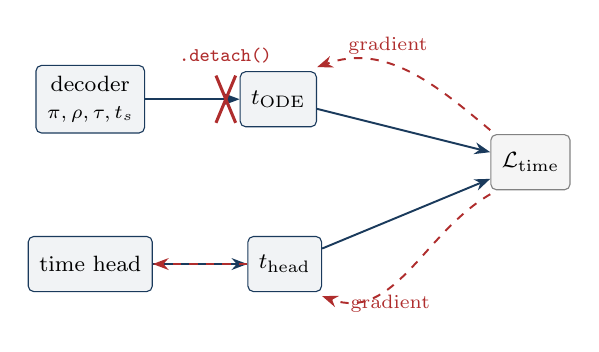
\begin{tikzpicture}[node distance=6mm and 12mm]
\node[blk] (dec) {decoder\\{\scriptsize$\pi,\rho,\tau,\ts$}};
\node[blk, right=of dec] (tode) {$t_{\text{ODE}}$};
\node[blk, below=13mm of dec] (head) {time head};
\node[blk, right=of head] (thead) {$t_{\text{head}}$};
\node[dat, right=22mm of tode, yshift=-8mm] (loss) {$\mathcal{L}_{\text{time}}$};

\draw[ar] (dec)  -- (tode);
\draw[ar] (head) -- (thead);
\draw[ar] (tode)  -- (loss);
\draw[ar] (thead) -- (loss);

% gradient paths
\draw[arg] ($(loss.north west)+(0,0.05)$) to[out=140,in=20]
   node[above, font=\scriptsize, cRed, pos=0.62] {gradient} ($(tode.north east)+(0,0.05)$);
\draw[arg] ($(loss.south west)+(0,-0.05)$) to[out=210,in=-20]
   node[below, font=\scriptsize, cRed, pos=0.62] {gradient} ($(thead.south east)+(0,-0.05)$);
\draw[arg] (thead) -- (head);

% the cut
\node[cRed, font=\small\bfseries] at ($(dec)!0.5!(tode)$) [yshift=-5.5mm] {};
\draw[cRed, line width=1.1pt] ($(tode.west)+(-0.30,-0.30)$) -- ($(tode.west)+(-0.05,0.30)$);
\draw[cRed, line width=1.1pt] ($(tode.west)+(-0.30,0.30)$) -- ($(tode.west)+(-0.05,-0.30)$);
\node[cRed, font=\scriptsize, anchor=south, align=center]
  at ($(tode.west)+(-0.18,0.34)$) {\texttt{.detach()}};
\end{tikzpicture}
\caption{The stop-gradient in Loss A. Solid arrows are the forward pass; dashed
red arrows are gradient flow during backpropagation. The gradient reaches
$t_{\text{head}}$ and continues into the head (and onward into $z$), but is
severed before it can reach the decoder. Only the student is allowed to move
toward the teacher.}
\label{fig:stopgrad}
\end{figure}

This asymmetry --- a one-directional teacher--student relationship enforced by a
stop-gradient --- is the same device used to prevent representational collapse
in self-supervised methods such as BYOL and SimSiam, in target networks for
value-based reinforcement learning, and in knowledge distillation. Here the ODE
branch is the teacher, not because it is correct, but because it is the branch
grounded in the reconstruction loss and therefore in the data.

\subsubsection{Loss B --- the ODE residual}
\label{sec:loss-b}

This is the highest-impact addition. Rather than regressing the head against a
derived signal, it takes the head's \emph{own} time, scales it to
$[0, \tmax]$, evaluates the ODE there, and compares to observation:
%
\begin{keybox}
\begin{equation}
\mathcal{L}_{\text{res}}
= \big\lVert \uns_{\text{ODE}}(t_i) - \uns_{\text{obs}} \big\rVert^2
+ \big\lVert \spl_{\text{ODE}}(t_i) - \spl_{\text{obs}} \big\rVert^2
\label{eq:ode-residual}
\end{equation}
\end{keybox}
%
The induction branch is evaluated at $\min(t_i, \ts)$ and the repression branch
at $(t_i - \ts)^{+}$, and the two are blended by a soft gate
$\sigma\big(5(\ts - t_i)\big)$ so that the branch switch is differentiable.
Residuals are normalised per gene so that all genes contribute equally.

Because gradients flow into the time head --- and onward into $z$, as noted in
Section~\ref{sec:time-head} --- the head is trained to find the time that best
\emph{explains the observed expression}. This is a differentiable analogue of
the expectation--maximisation time step used by scVelo, and it is the component
to which the ablation attributes most of the pseudotime improvement
($0.33 \to 0.75$ Spearman).

\paragraph{Why there is no stop-gradient here.} Loss B contains no
\texttt{detach} anywhere along the path
$\mathcal{L}_{\text{res}} \to t_i \to \text{head} \to z \to \text{encoder}$,
and this is deliberate. The distinction from Loss A lies entirely in what the
target is: here the comparison is against $\uns_{\text{obs}}$ and
$\spl_{\text{obs}}$, which are \emph{observed data} --- constants with no
parameters behind them. There is nothing to corrupt and no degenerate solution
to collapse into, so unrestricted gradient flow is exactly what is wanted. It
is what allows this loss to reach the encoder and reorganise the latent space.
The governing rule is therefore simple:

\begin{keybox}
\textbf{Detach when the target is produced by the model. Do not when the target
is data.}
\end{keybox}

\subsubsection{The stop-gradient pattern elsewhere in the model}

The same reasoning recurs in three further places, following a consistent
principle: \emph{detach the selection or the weighting, retain gradient on the
quantity actually being compared.}

\begin{lstlisting}
# velocity-time consistency: the pair weights are frozen
time_diff = (t_j_final - t_i_final).detach()
weights   = torch.clamp(time_diff / (time_diff.mean() + 1e-8), 0, 3)
\end{lstlisting}

Without this detach the model could reduce the loss by shrinking all latent-time
gaps rather than by correcting velocity directions --- satisfying the objective
by manipulating the weights instead of by meeting the constraint.

\begin{lstlisting}
# temporal smoothness and velocity coherence: neighbour choice is frozen
with torch.no_grad():
    dists = torch.cdist(z.detach(), z.detach())
    _, nn_idx = dists.topk(k, largest=False)
\end{lstlisting}

Selecting the $k$ nearest neighbours is a discrete operation; differentiating
through the choice itself is meaningless. The gradient belongs on the times and
velocities being compared, not on which cells happened to be selected.

\subsubsection{Geometric regularisers}

Two further terms impose structure rather than fitting data. The
\textbf{velocity--time consistency} loss samples random cell pairs, orders them
so that $t_i < t_j$, and penalises velocity that points backwards:
%
\begin{equation}
\mathcal{L}_{\text{vtc}} = \operatorname{ReLU}\!\Big(-\cos\big(v_i,\ \spl_j - \spl_i\big)\Big),
\end{equation}
%
weighted by the time gap. The \textbf{temporal smoothness} loss takes the ten
nearest neighbours in latent space and penalises squared time differences:
%
\begin{equation}
\mathcal{L}_{\text{ts}} = \frac{1}{k}\sum_{j \in \mathcal{N}(i)} \big(t_i - t_j\big)^2 .
\end{equation}

%======================================================================
\section{Inference}
\label{sec:inference}
%======================================================================

\subsection{Computing velocity}

For each of $25$ posterior samples, the procedure is:

\begin{enumerate}[leftmargin=*]
\item forward pass, giving $\alpha_{ig}, \beta, \gamma, \pi, \rho, \tau$;
\item evaluate the ODE at each state's time to obtain \emph{model-predicted}
      $\uns, \spl$ --- not the observed counts. This is the denoising step, and
      it is the reason the estimate is smooth;
\item compute per-state velocities
      $v_{\text{ind}} = \beta \uns_{\text{ind}} - \gamma \spl_{\text{ind}}$,
      $v_{\text{rep}} = \beta \uns_{\text{rep}} - \gamma \spl_{\text{rep}}$, and
      $v_{\text{steady}} = 0$ (by definition, nothing changes at a plateau);
\item take the expectation under the state probabilities,
      \begin{equation}
      v = \pi_{\text{ind}} v_{\text{ind}} + \pi_{\text{rep}} v_{\text{rep}}
          + \pi_{\text{steady}} \cdot 0 ;
      \end{equation}
\item clip so that $v \ge -\spl$, ensuring predicted future abundance cannot
      become negative;
\item optionally smooth over the $k$NN graph,
      $v \leftarrow (1-a) v + a\,(Wv)$ with $a = 0.5$ and $W$ row-normalised.
\end{enumerate}

Averaging over posterior samples turns the sampled $z$ into a Monte Carlo
estimate of $\E[v]$, and the spread across samples is a usable uncertainty
measure.

\subsection{Three distinct notions of time}

The model contains three time-like quantities which are easily confused. They
live on different axes and answer different questions.

\begin{table}[h]
\centering
\caption{The three time quantities.}
\label{tab:times}
\small
\begin{tabular}{@{}p{2.3cm}p{3.9cm}p{3.9cm}p{4.4cm}@{}}
\toprule
 & \texttt{learned\_time} $t_i$ & switch time $\ts$ & velocity pseudotime $t_{\text{VPT}}$ \\
\midrule
Shape   & $[N]$ --- per \emph{cell} & $[G]$ --- per \emph{gene} & $[N]$ --- per \emph{cell} \\
Range   & $[0,1]$ & $[0, \tmax]$, with $\tmax = 20$ & $[0,1]$ after normalisation \\
Kind    & variable, computed per cell & parameter, shared by all cells & post-hoc graph computation \\
Source  & $\sigma(\mathrm{MLP}(z))$ & clamped $\softplus(\theta_s)$ & diffusion pseudotime on the velocity graph \\
Answers & how far along the trajectory is this \emph{cell}? & when does this \emph{gene} stop being induced? & how far downstream of the source is this \emph{cell}? \\
\bottomrule
\end{tabular}
\end{table}

\subsubsection{How \texorpdfstring{$t_i$}{t\_i} and \texorpdfstring{$\ts$}{t\_s} combine}

The two are orthogonal, and their interaction is the mechanism by which a
single cell-level clock can describe a thousand genes with different dynamics.
A cell axis of length $N$ is broadcast against a gene axis of length $G$:
%
\begin{equation}
\text{gate}_{ig} = \sigma\Big(5\big(\ts^{(g)} - \tmax \cdot t_i\big)\Big) \in [0,1],
\end{equation}
%
which asks, for every (cell, gene) pair: \emph{has this cell's clock passed this
gene's switch point?} If so the gene is repressing in that cell; if not it is
still inducing.

\begin{keybox}
\textbf{Example.} Take a cell with $t_i = 0.5$, so its clock reads $10$ on the
$[0, 20]$ scale.

\medskip
\begin{center}
\begin{tabular}{@{}lccl@{}}
\toprule
Gene & $\ts$ & comparison & state \emph{in this cell} \\
\midrule
A & $5$  & $10 > 5$    & already repressing \\
B & $15$ & $10 < 15$   & still inducing \\
C & $10$ & $10 \approx 10$ & at its peak \\
\bottomrule
\end{tabular}
\end{center}
\medskip

One cell, one clock, three different gene states --- because each gene carries
its own switch point. Genes turn off at different stages of the same shared
trajectory, and that staggering is what constitutes a differentiation cascade.
\end{keybox}

\begin{figure}[htbp]
\centering
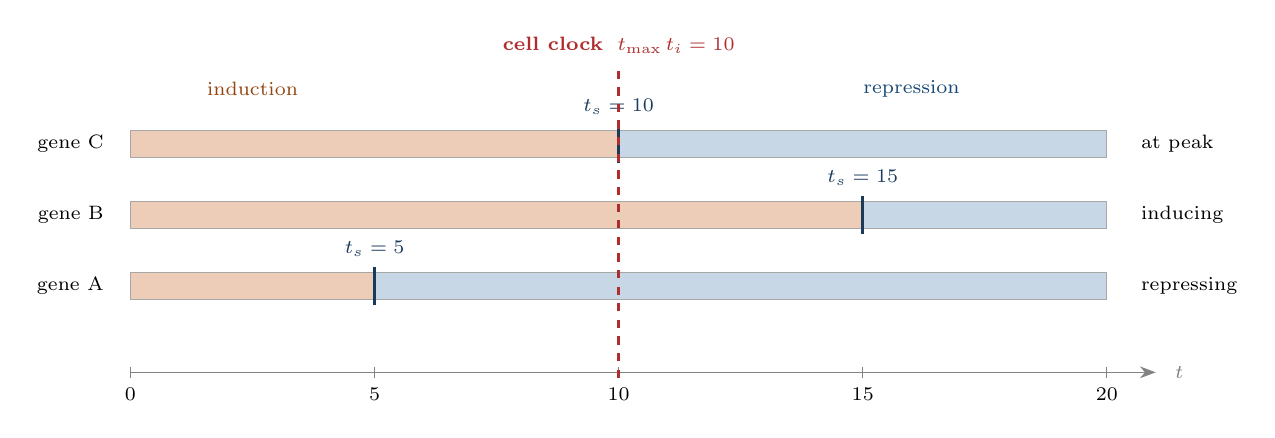
\begin{tikzpicture}[x=0.62cm, y=1cm]
% axis
\draw[-{Stealth[length=2mm]}, draw=cGrey] (0,-0.55) -- (21,-0.55);
\foreach \x in {0,5,10,15,20}
  \draw[draw=cGrey] (\x,-0.48) -- (\x,-0.62) node[below, font=\scriptsize] {\x};
\node[font=\scriptsize, cGrey, anchor=west] at (21.2,-0.55) {$t$};

% gene bars: {name}{ts}{y}
\foreach \g/\tsw/\yy in {A/5/0.55, B/15/1.45, C/10/2.35} {
  \fill[cU!30] (0,\yy-0.17) rectangle (\tsw,\yy+0.17);
  \fill[cS!25] (\tsw,\yy-0.17) rectangle (20,\yy+0.17);
  \draw[draw=cGrey!70] (0,\yy-0.17) rectangle (20,\yy+0.17);
  \draw[tarvinavy, line width=1pt] (\tsw,\yy-0.24) -- (\tsw,\yy+0.24);
  \node[font=\scriptsize, anchor=east] at (-0.35,\yy) {gene \g};
  \node[font=\scriptsize, tarvinavy, anchor=south] at (\tsw,\yy+0.25) {$\ts=\tsw$};
}
\node[font=\scriptsize, cU!75!black] at (2.5,3.05) {induction};
\node[font=\scriptsize, cS!75!black] at (16,3.05) {repression};

% the cell clock
\draw[cRed, line width=1.2pt, dashed] (10,-0.62) -- (10,3.35);
\node[cRed, font=\scriptsize\bfseries, anchor=south] at (10,3.38)
  {cell clock $\;\tmax\, t_i = 10$};

% verdicts
\node[font=\scriptsize, anchor=west] at (20.5,0.55) {repressing};
\node[font=\scriptsize, anchor=west] at (20.5,1.45) {inducing};
\node[font=\scriptsize, anchor=west] at (20.5,2.35) {at peak};
\end{tikzpicture}
\caption{One cell-level clock, three gene-level switch points. The red line is
this cell's time, a single number shared by every gene. Each bar is one gene's
own life cycle, split at its own $\ts$. Where the red line falls within a bar
determines that gene's state \emph{in this cell} --- which is how a single
scalar per cell can describe genes with entirely different dynamics.}
\label{fig:clock}
\end{figure}

\subsubsection{Obtaining \texorpdfstring{$t_i$}{t\_i} at inference}

Retrieving the learned time requires only the encoder and the time head; the
decoder, the ODE and the TF module are untouched, which is why it is
inexpensive:

\begin{lstlisting}
for tensors in scdl:                          # minibatches of cells
    sample_times = []
    for _ in range(n_samples):                # 25 posterior draws
        inference_outputs, _ = self.module.forward(tensors, compute_loss=False)
        sample_times.append(inference_outputs["learned_time"].cpu().numpy())
    all_times.append(np.mean(sample_times, axis=0))
\end{lstlisting}

Because $z$ is \emph{sampled} from $q(z \mid \spl, \uns)$ rather than taken at its
mean, each pass yields a slightly different $t$. Averaging is Monte Carlo
estimation of the posterior mean:
%
\begin{equation}
\hat{t}_i \;=\; \E_{z \sim q(z \mid \spl_i, \uns_i)}\big[\,\mathrm{head}(z)\,\big]
\;\approx\; \frac{1}{25}\sum_{k=1}^{25} \mathrm{head}\big(z^{(k)}\big).
\end{equation}

\subsection{Contribution 3: velocity--pseudotime blending}

\subsubsection{Computing \texorpdfstring{$t_{\text{VPT}}$}{t\_VPT}}

Velocity pseudotime is a cell ordering derived from the velocity field itself.
It is computed after training, as post-processing, in four steps.

\paragraph{Step 1: the velocity graph.} For every cell $i$ and each neighbour
$j$, compare where cell $i$ is pointing against where cell $j$ actually lies:
%
\begin{equation}
\pi_{ij} = \cos\big(v_i,\ \spl_j - \spl_i\big)
= \frac{v_i \cdot (\spl_j - \spl_i)}{\lVert v_i \rVert\, \lVert \spl_j - \spl_i \rVert}.
\end{equation}
%
A high value means $i$'s velocity points directly at $j$, making $j$ a
plausible next state. The resulting matrix is \emph{asymmetric}, and that
asymmetry is the entire source of directionality.

\paragraph{Step 2: transition probabilities.} Exponentiate and row-normalise
over neighbours,
%
\begin{equation}
P_{ij} = \frac{\exp(\sigma \pi_{ij})}{\sum_{k \in \mathcal{N}(i)} \exp(\sigma \pi_{ik})},
\end{equation}
%
turning the velocity field into a directed Markov chain over cells.

\paragraph{Step 3: diffusion pseudotime.} A root cell is inferred from the
spectral structure of $P$ --- roughly, the cell from which flow originates ---
and diffusion pseudotime is computed as the diffusion distance from that root.
The essential point is that the ordering derives from \emph{velocity
directions}: ordinary diffusion pseudotime on a $k$NN graph yields an
undirected ordering with no way to identify which end is the beginning.
Velocity supplies the arrow of time.

\paragraph{Step 4: normalisation and blending.} The result is scaled to
$[0,1]$, the learned time is sign-aligned against it, and the two are averaged:

\begin{lstlisting}
corr, _ = spearmanr(learned_t, vpt_norm)
if corr < 0:
    learned_t = 1.0 - learned_t          # sign alignment
latent_time = blend * vpt_norm + (1 - blend) * learned_t   # blend = 0.5
\end{lstlisting}

The sign alignment is necessary because a pseudotime without a root is defined
only up to reversal; $t_{\text{VPT}}$ has an inferred root, so its direction is
treated as canonical.

\subsubsection{Why blending helps}

\begin{center}
\begin{tabular}{@{}lll@{}}
\toprule
 & \textbf{Global direction} & \textbf{Local smoothness} \\
\midrule
$t_{\text{VPT}}$      & yes --- has a root, follows the flow & no --- jagged on a sparse noisy graph \\
\texttt{learned\_time} & no --- can drift without an anchor  & yes --- a smooth function of $z$ \\
\bottomrule
\end{tabular}
\end{center}

Each component compensates for the other's failure mode. The two are produced
by entirely independent mechanisms --- a per-cell regression and a global
diffusion process --- so their errors are largely uncorrelated and averaging
cancels noise rather than reinforcing it.

Note also that $t_{\text{VPT}}$ is computed \emph{from} TARVI's velocity, so
the quality of Contribution 3 depends directly on Contributions 1 and 2. The
three do not merely add; they compound.

%======================================================================
\section{Evaluation}
%======================================================================

Training uses no ground truth. Evaluation deliberately does, and holds it out
entirely from the fitting procedure:

\begin{itemize}[leftmargin=*]
\item \textbf{Cell-type annotations} support cross-boundary direction accuracy
      (CBDir), which checks that velocity points from progenitor to descendant
      across known lineage boundaries.
\item \textbf{Known developmental ordering} allows pseudotime to be scored by
      rank correlation.
\item \textbf{Measured time} exists for the scEU-seq organoid dataset via
      metabolic labelling, and is consumed directly by the ground-truth
      temporal metrics.
\end{itemize}

Additional metric families cover velocity confidence and coherence length,
gene-level velocity $R^2$, state-assignment entropy and purity, and transition
probability scores. Benchmarking is against velocyto, scVelo in both
deterministic and dynamical modes, and VeloVI, across five datasets, with a
four-mode component ablation.

\begin{keybox}
The methodological point is that ground truth is available but is
\emph{deliberately excluded} from training. Had the labels been used to fit the
model, the benchmark numbers would carry no information.
\end{keybox}

\section*{Summary of results}
\addcontentsline{toc}{section}{Summary of results}

\begin{table}[h]
\centering
\caption{Cross-dataset means over five datasets. Higher is better throughout.}
\begin{tabular}{@{}lcccccc@{}}
\toprule
\textbf{Method} & CBDir & VelConf & PT-Spear & PT-DistCorr & PT-Cons & Gene-$R^2$ \\
\midrule
\textbf{TARVI} & \textbf{0.933} & \textbf{0.927} & \textbf{0.747} & \textbf{0.771} & \textbf{0.986} & \textbf{0.477} \\
VeloVI         & 0.931 & 0.920 & 0.331 & 0.341 & 0.904 & 0.443 \\
\bottomrule
\end{tabular}
\end{table}

TARVI matches the strongest baseline on cross-boundary direction accuracy while
substantially improving pseudotime calibration, a $126\%$ relative gain in
Spearman correlation over VeloVI.

%======================================================================
\appendix
\section{Notation and tensor shapes}
\label{app:notation}
%======================================================================

\begin{center}
\begin{tabular}{@{}llp{8.2cm}@{}}
\toprule
\textbf{Symbol} & \textbf{Shape} & \textbf{Meaning} \\
\midrule
$N$, $G$, $T$ & --- & number of cells, genes, transcription factors \\
$\uns$, $\spl$ & $[N, G]$ & unspliced and spliced abundance (moments, scaled) \\
$\alpha$ & $[N, G]$ & transcription rate; cell-specific under TF regulation \\
$\beta$, $\gamma$ & $[G]$ & splicing and degradation rate, per gene \\
$v$ & $[N, G]$ & RNA velocity, $\beta \uns - \gamma \spl$ \\
\midrule
$z$ & $[N, 10]$ & latent cell state \\
$\mu_z$, $\sigma_z^2$ & $[N, 10]$ & variational posterior parameters \\
\midrule
$\pi$ & $[N, G, 4]$ & kinetic state weights (Dirichlet) \\
$\rho$ & $[N, G]$ & fractional progress through induction \\
$\tau$ & $[N, G]$ & fractional progress through repression \\
$\ts$ & $[G]$ & per-gene switch time \\
$\tmax$ & scalar & time horizon, fixed at $20$ \\
$t_i$ & $[N]$ & learned per-cell latent time, in $[0,1]$ \\
$t_{\text{VPT}}$ & $[N]$ & velocity pseudotime \\
\midrule
$M$ & $[G, T]$ & binary TF--target mask from ENCODE and ChEA \\
$W$ & $[G, T]$ & learnable TF--target weights \\
$b$ & $[G]$ & basal transcription rate \\
\bottomrule
\end{tabular}
\end{center}

\section{Where each component lives in the code}

\begin{center}
\begin{tabular}{@{}ll@{}}
\toprule
\textbf{Component} & \textbf{Location} \\
\midrule
Preprocessing, $k$NN velocity smoothing & \texttt{tarvi/\_utils.py} \\
TF mask construction, cell-specific $\alpha$ & \texttt{tarvi/\_tf\_module.py} \\
Encoder, decoder, ODE solutions, all losses & \texttt{tarvi/\_module.py} \\
Model class, velocity and time getters, VPT & \texttt{tarvi/\_model.py} \\
Graph-attention velocity refiner & \texttt{tarvi/\_gnn.py} \\
Benchmark metrics & \texttt{evaluation/metrics.py} \\
Training, benchmarking, ablation scripts & \texttt{scripts/} \\
\bottomrule
\end{tabular}
\end{center}

\end{document}
